\part{Conception applicative détaillée}

\section{Identification des services et la dynamique de l’architecture}


\subsection{CU1 - Génération de contacts}
\begin{figure}[H]
\noindent\makebox[\textwidth]{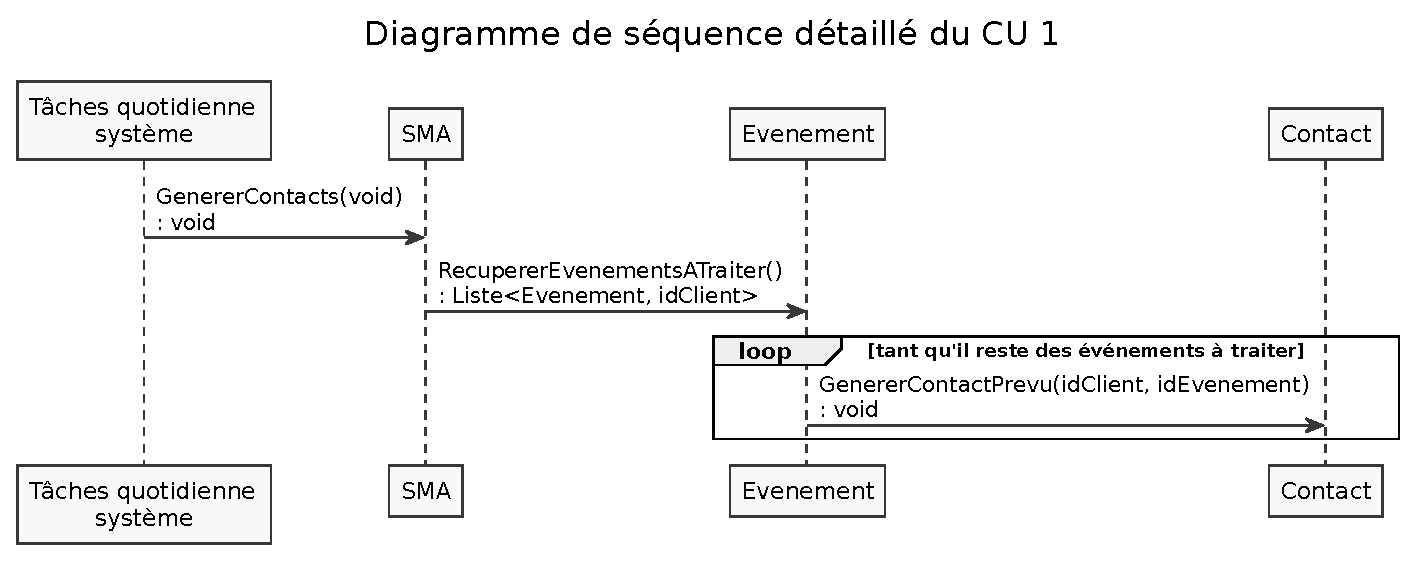
\includegraphics[width=19cm]{figures/eps/DSD_CU1.eps}}
\caption{DSD du CU1}
\end{figure}

\subsection{CU2 - Répartition des contacts commerciaux}
\begin{figure}[H]
\noindent\makebox[\textwidth]{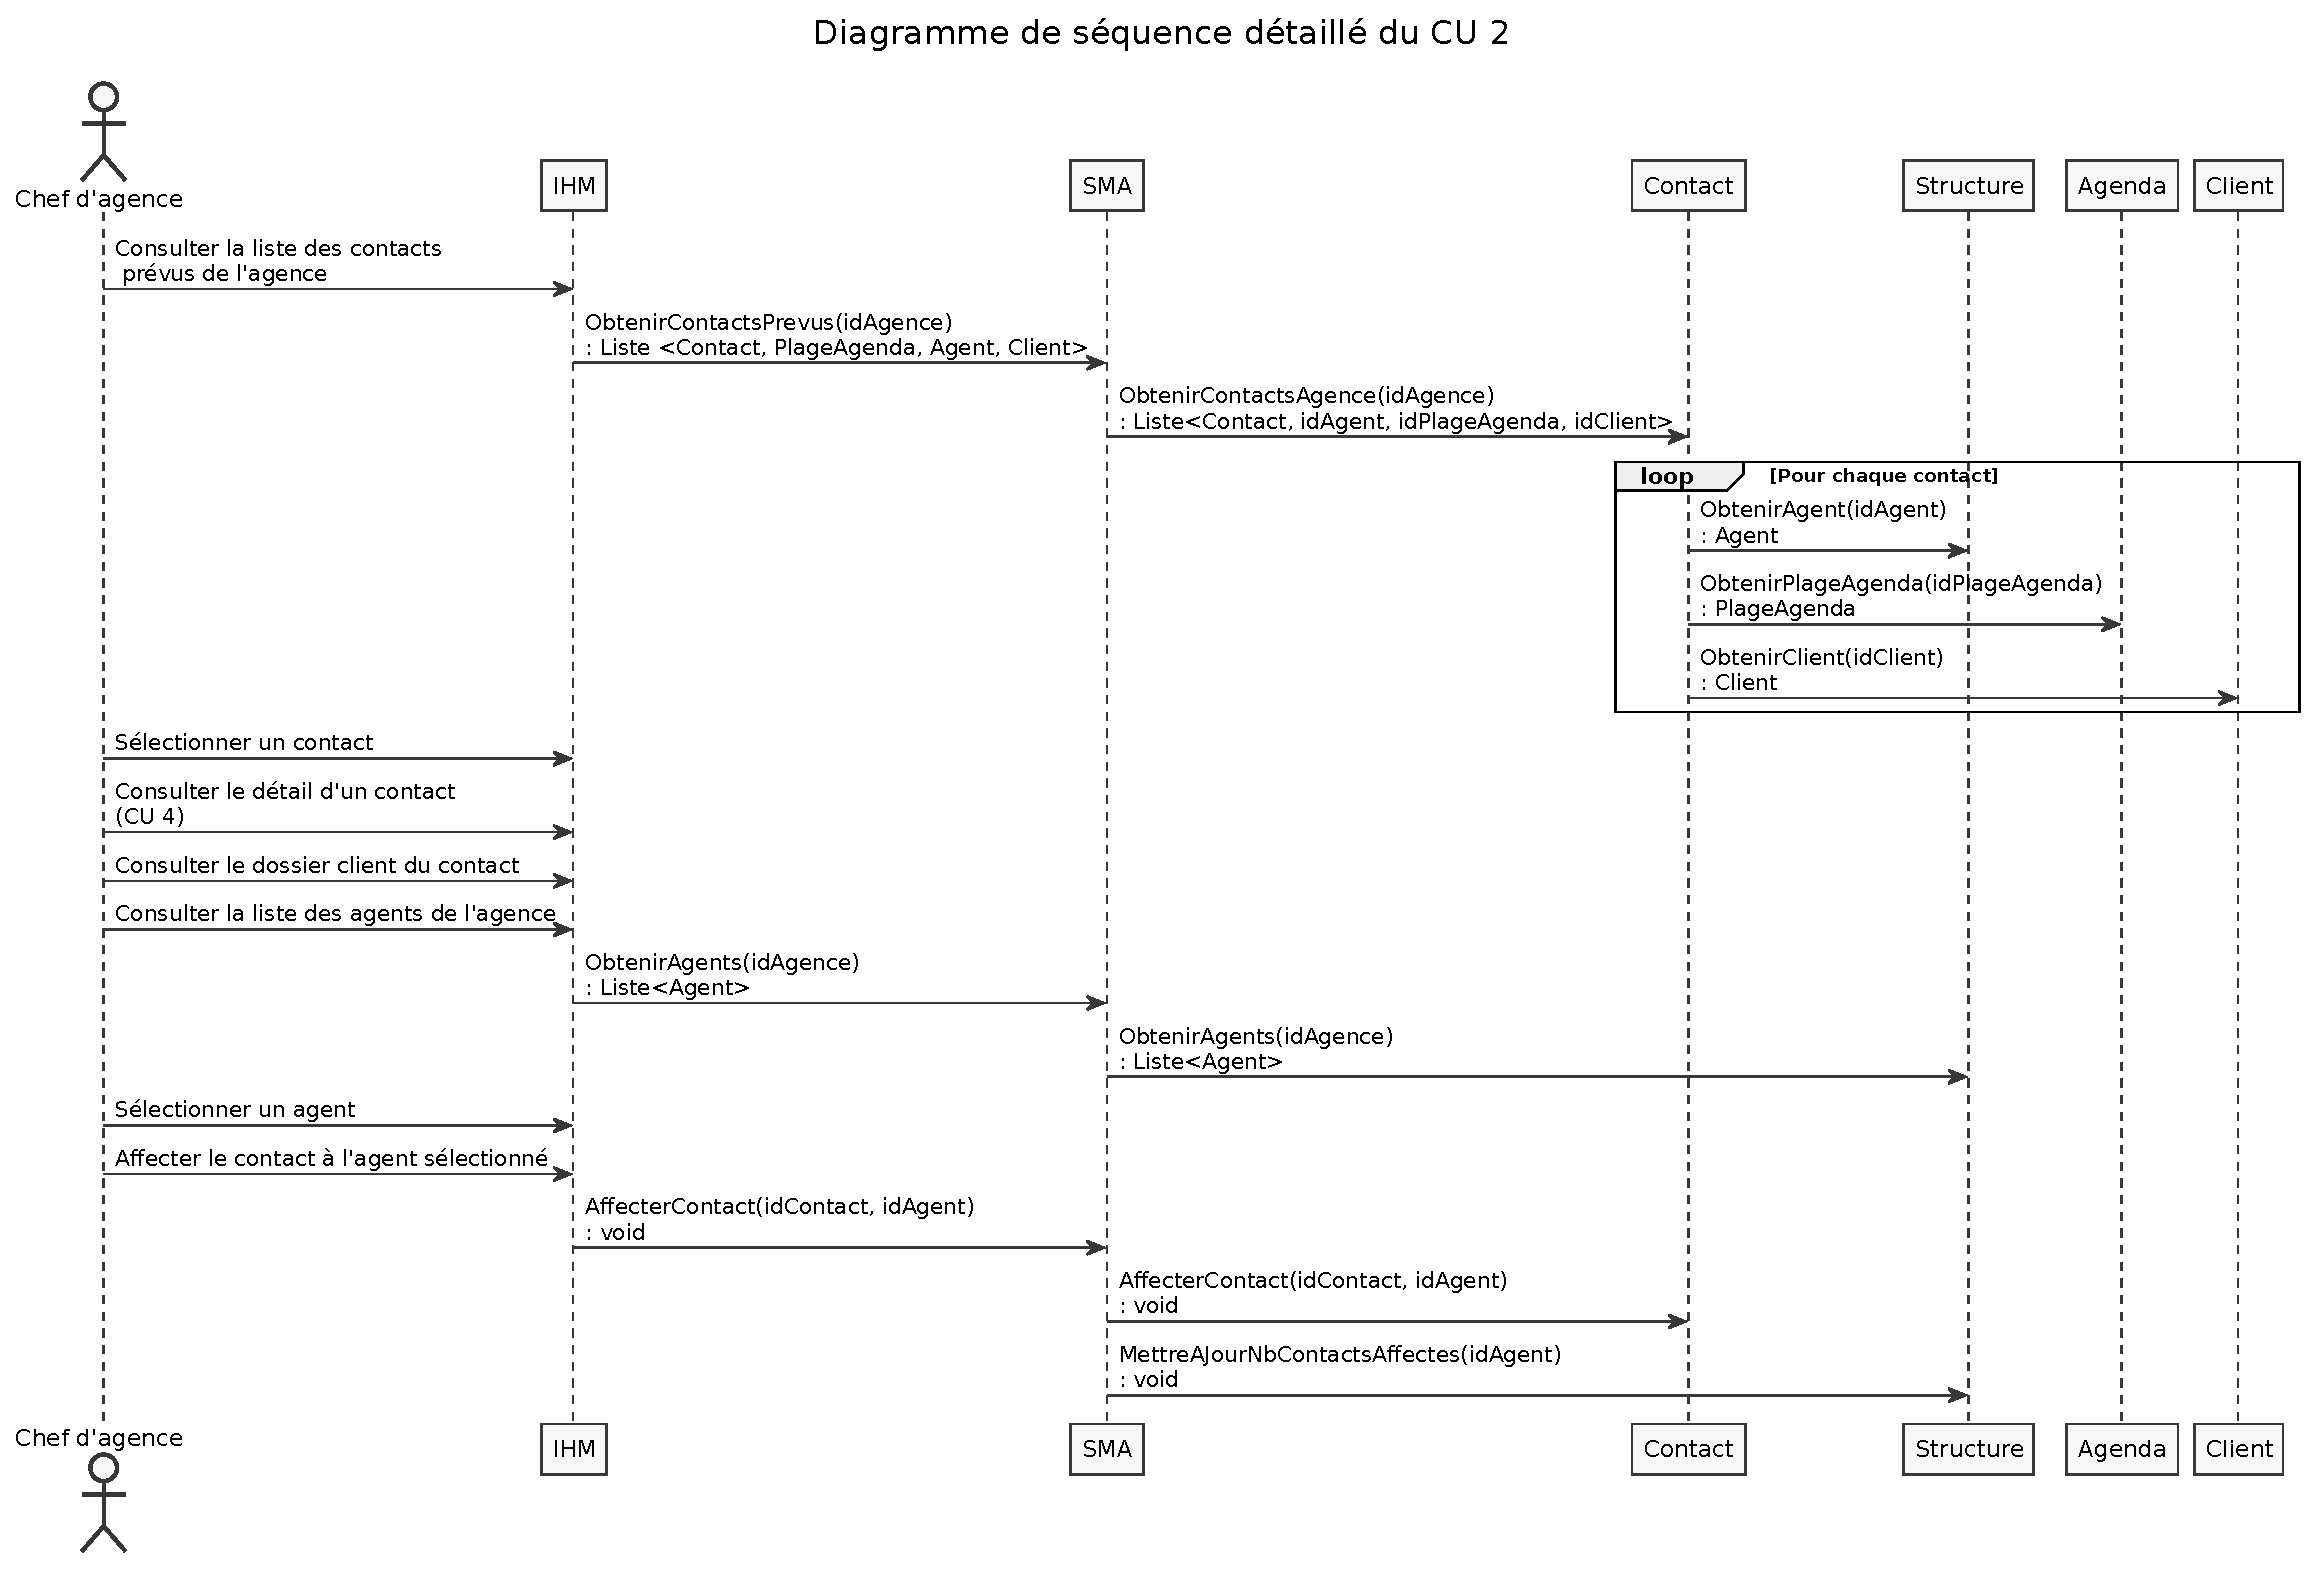
\includegraphics[width=23cm, angle=90]{figures/eps/DSD_CU2.eps}}
\caption{DSD du CU2}
\end{figure}


\subsection{CU3 - Suivi de l’action commercial}
\begin{figure}[H]
\noindent\makebox[\textwidth]{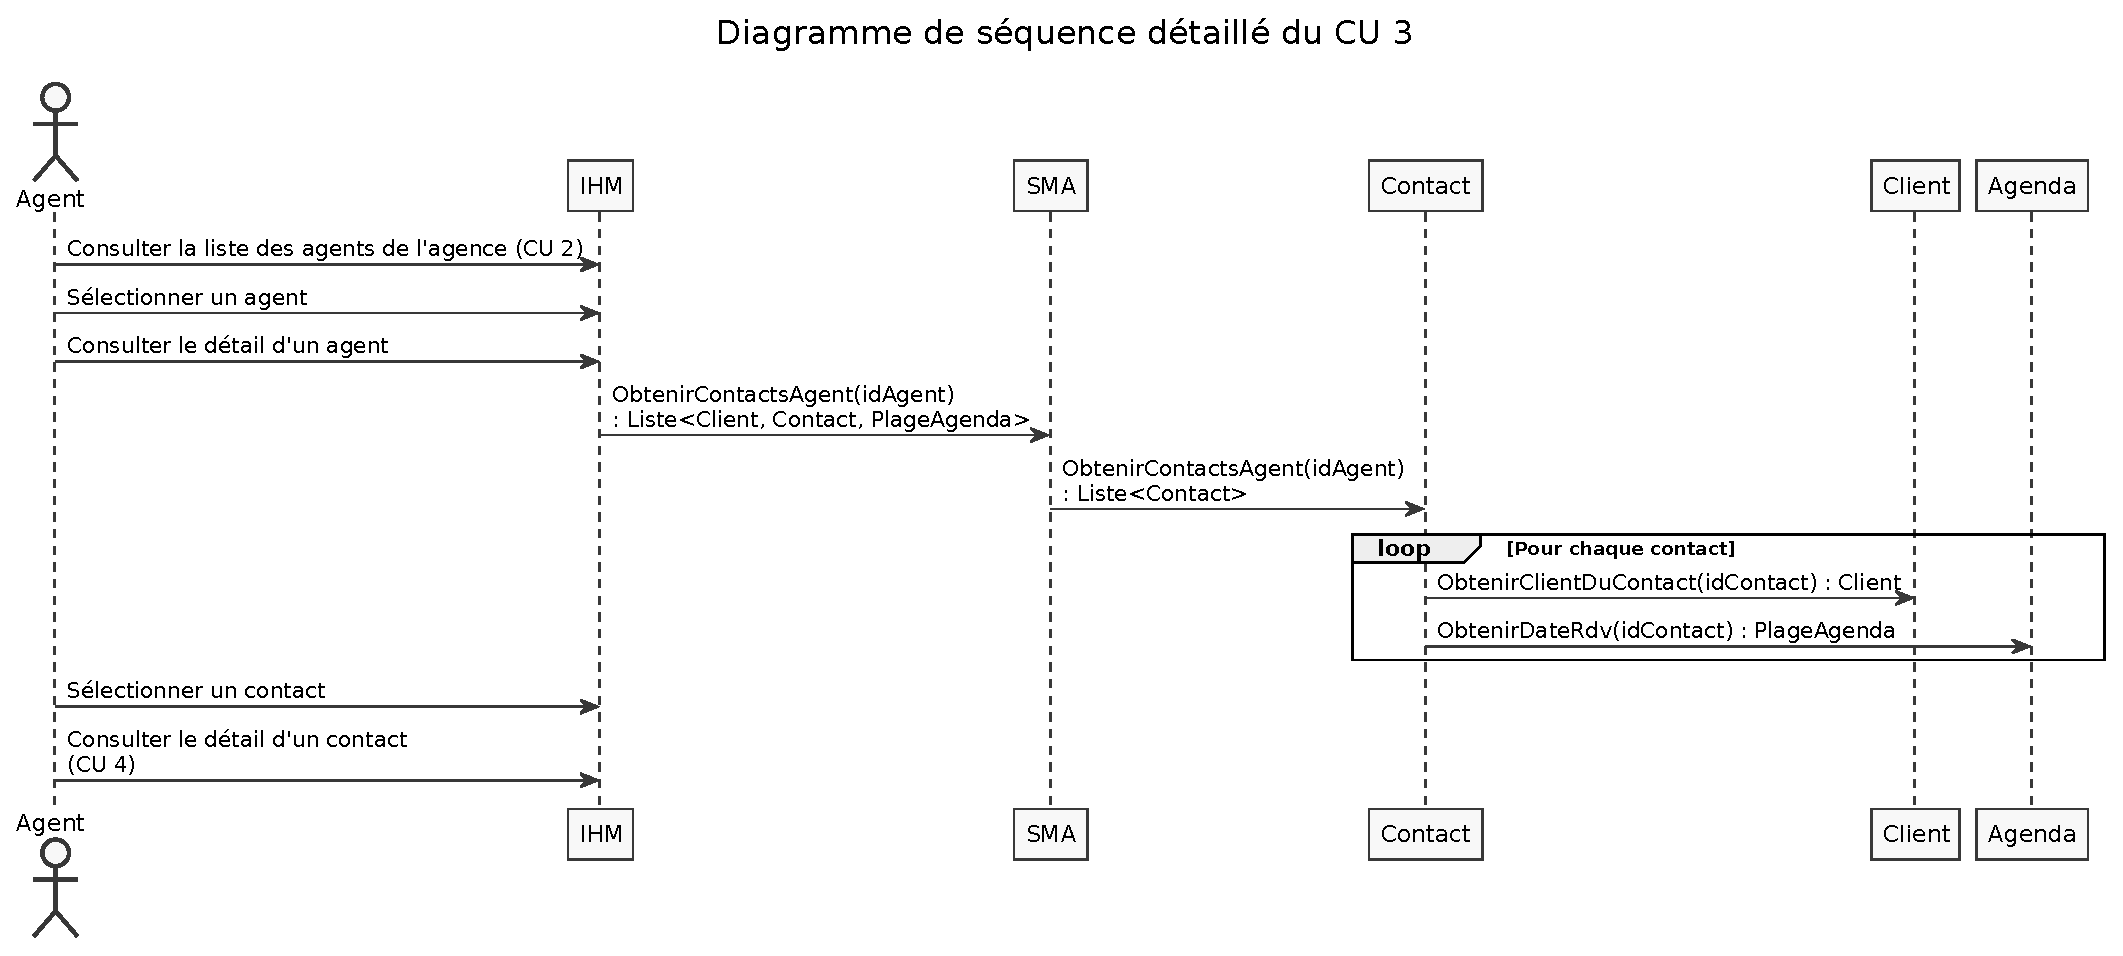
\includegraphics[width=21cm, angle=90]{figures/eps/DSD_CU3.eps}}
\caption{DSD du CU3}
\end{figure}

\subsection{CU4 – Gestion de la liste des contacts clients}
\begin{figure}[H]
\noindent\makebox[\textwidth]{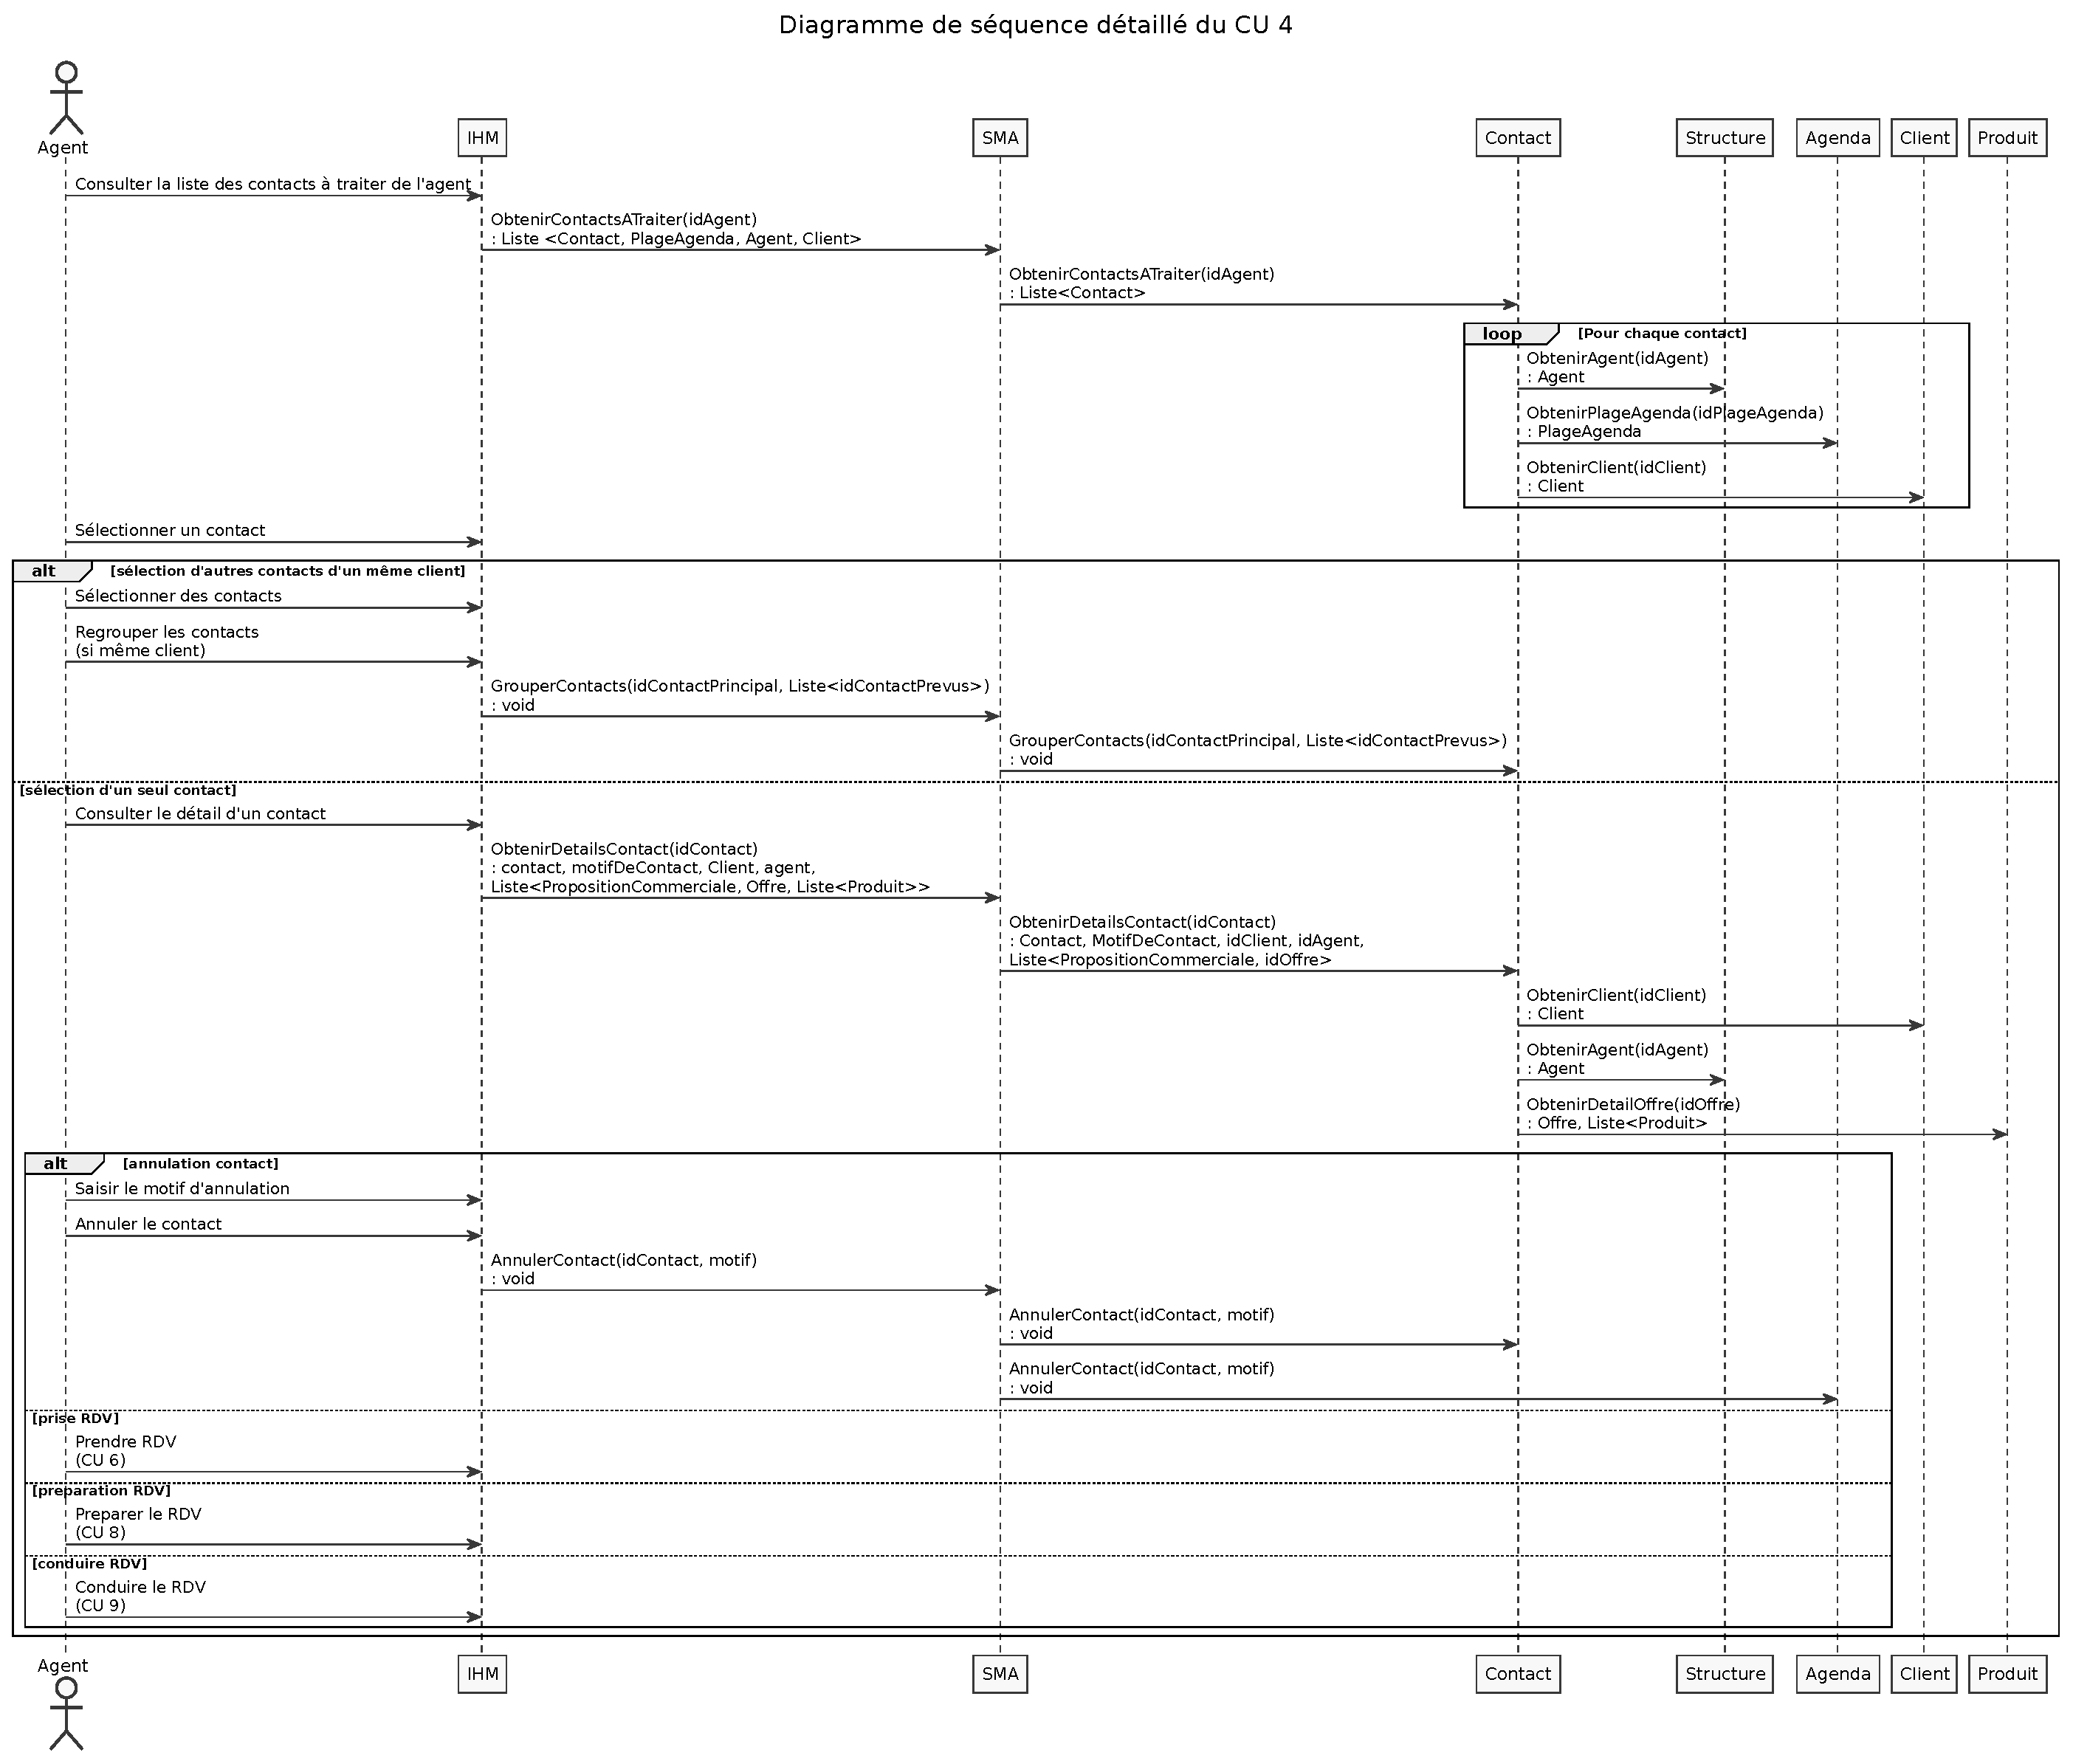
\includegraphics[width=20cm, angle=90]{figures/eps/DSD_CU4.eps}}
\caption{DSD du CU4}
\end{figure}


\subsection{CU5 - Planification de l’activité de l’agence du mois suivant}
\begin{figure}[H]
\noindent\makebox[\textwidth]{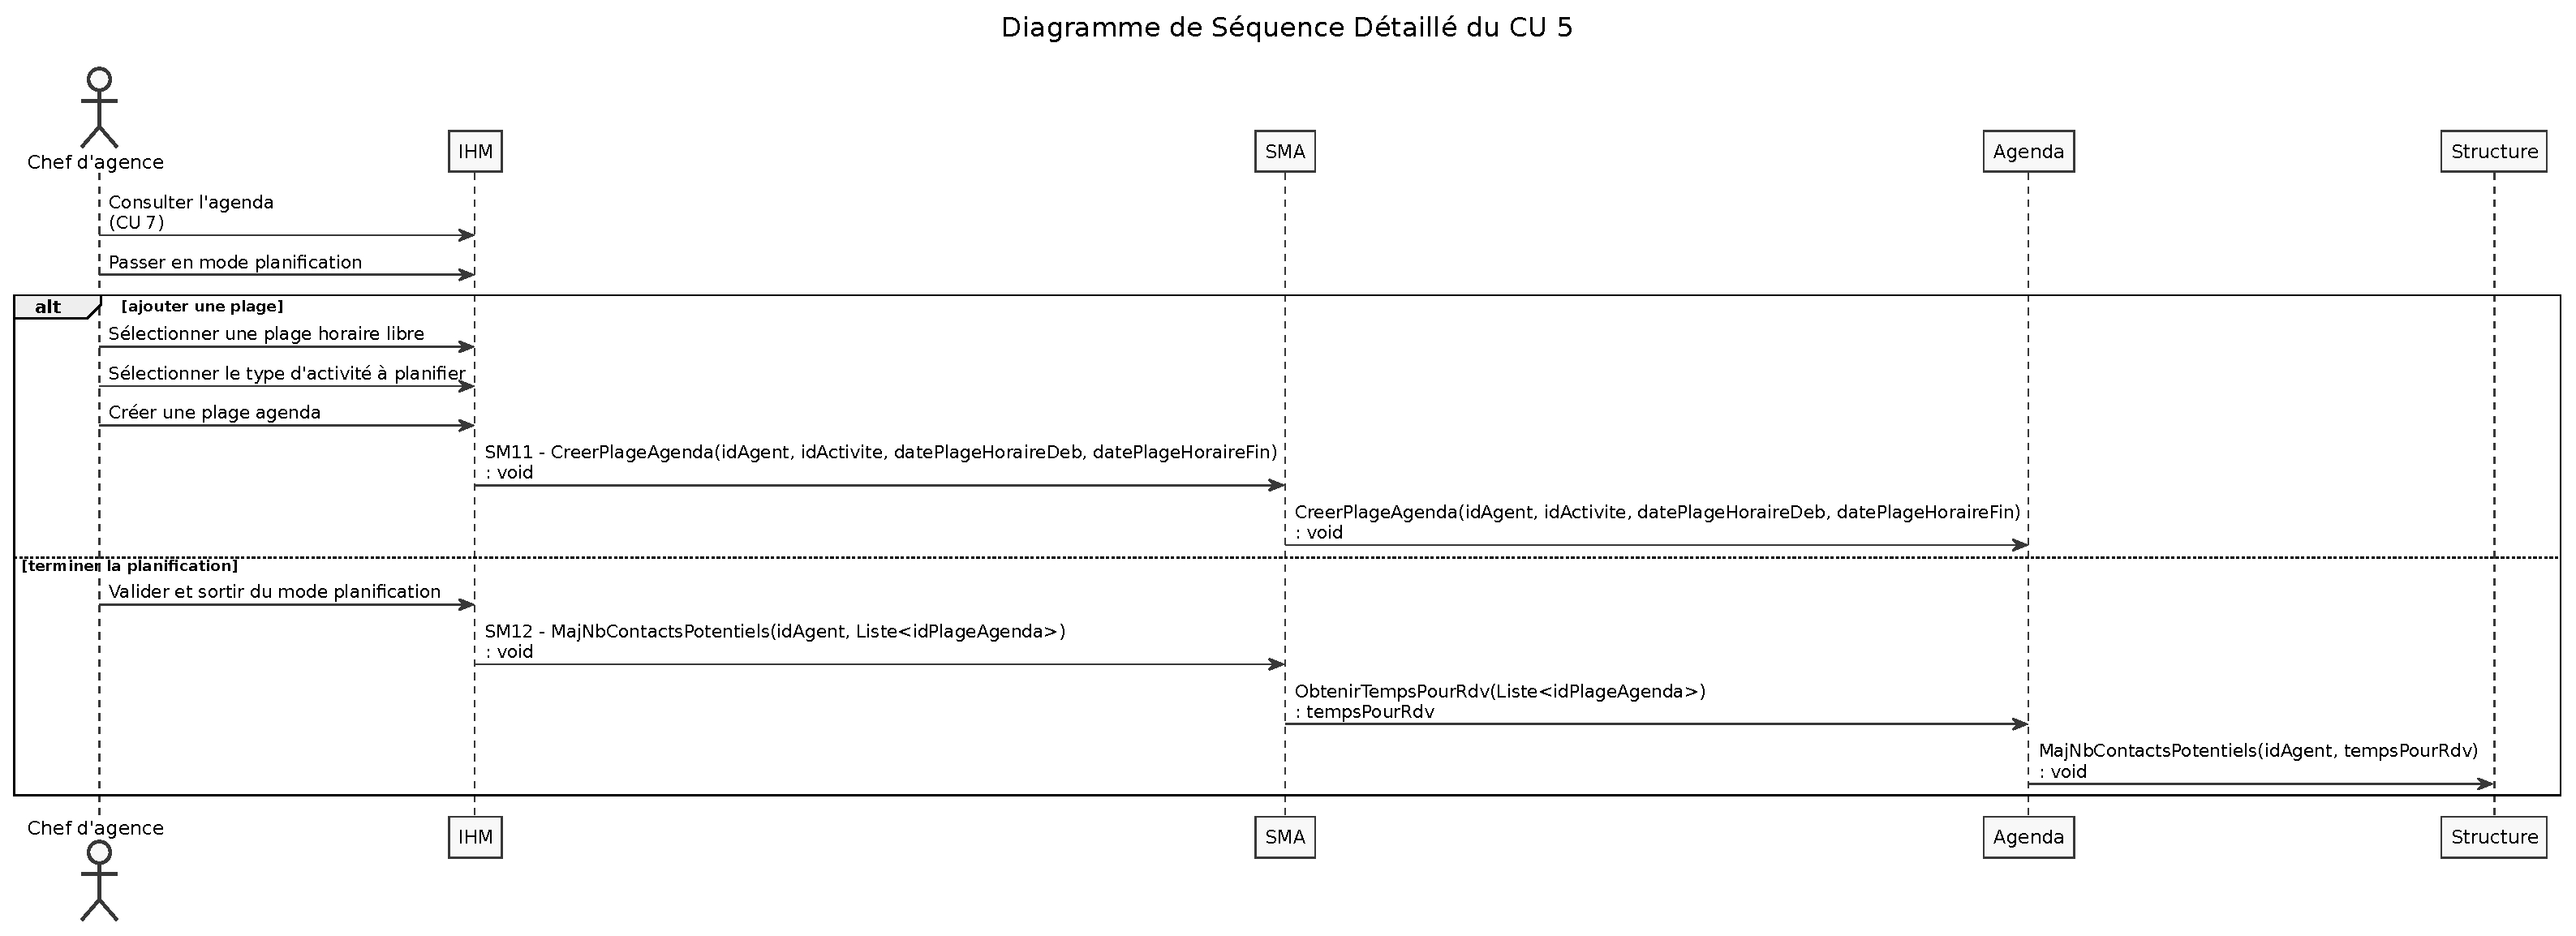
\includegraphics[width=24cm, angle=90]{figures/eps/DSD_CU5.eps}}
\caption{DSD du CU5}
\end{figure}


\subsection{CU6 - Planification des contacts commerciaux}

\subsubsection{contacts commerciaux}
\begin{figure}[H]
\noindent\makebox[\textwidth]{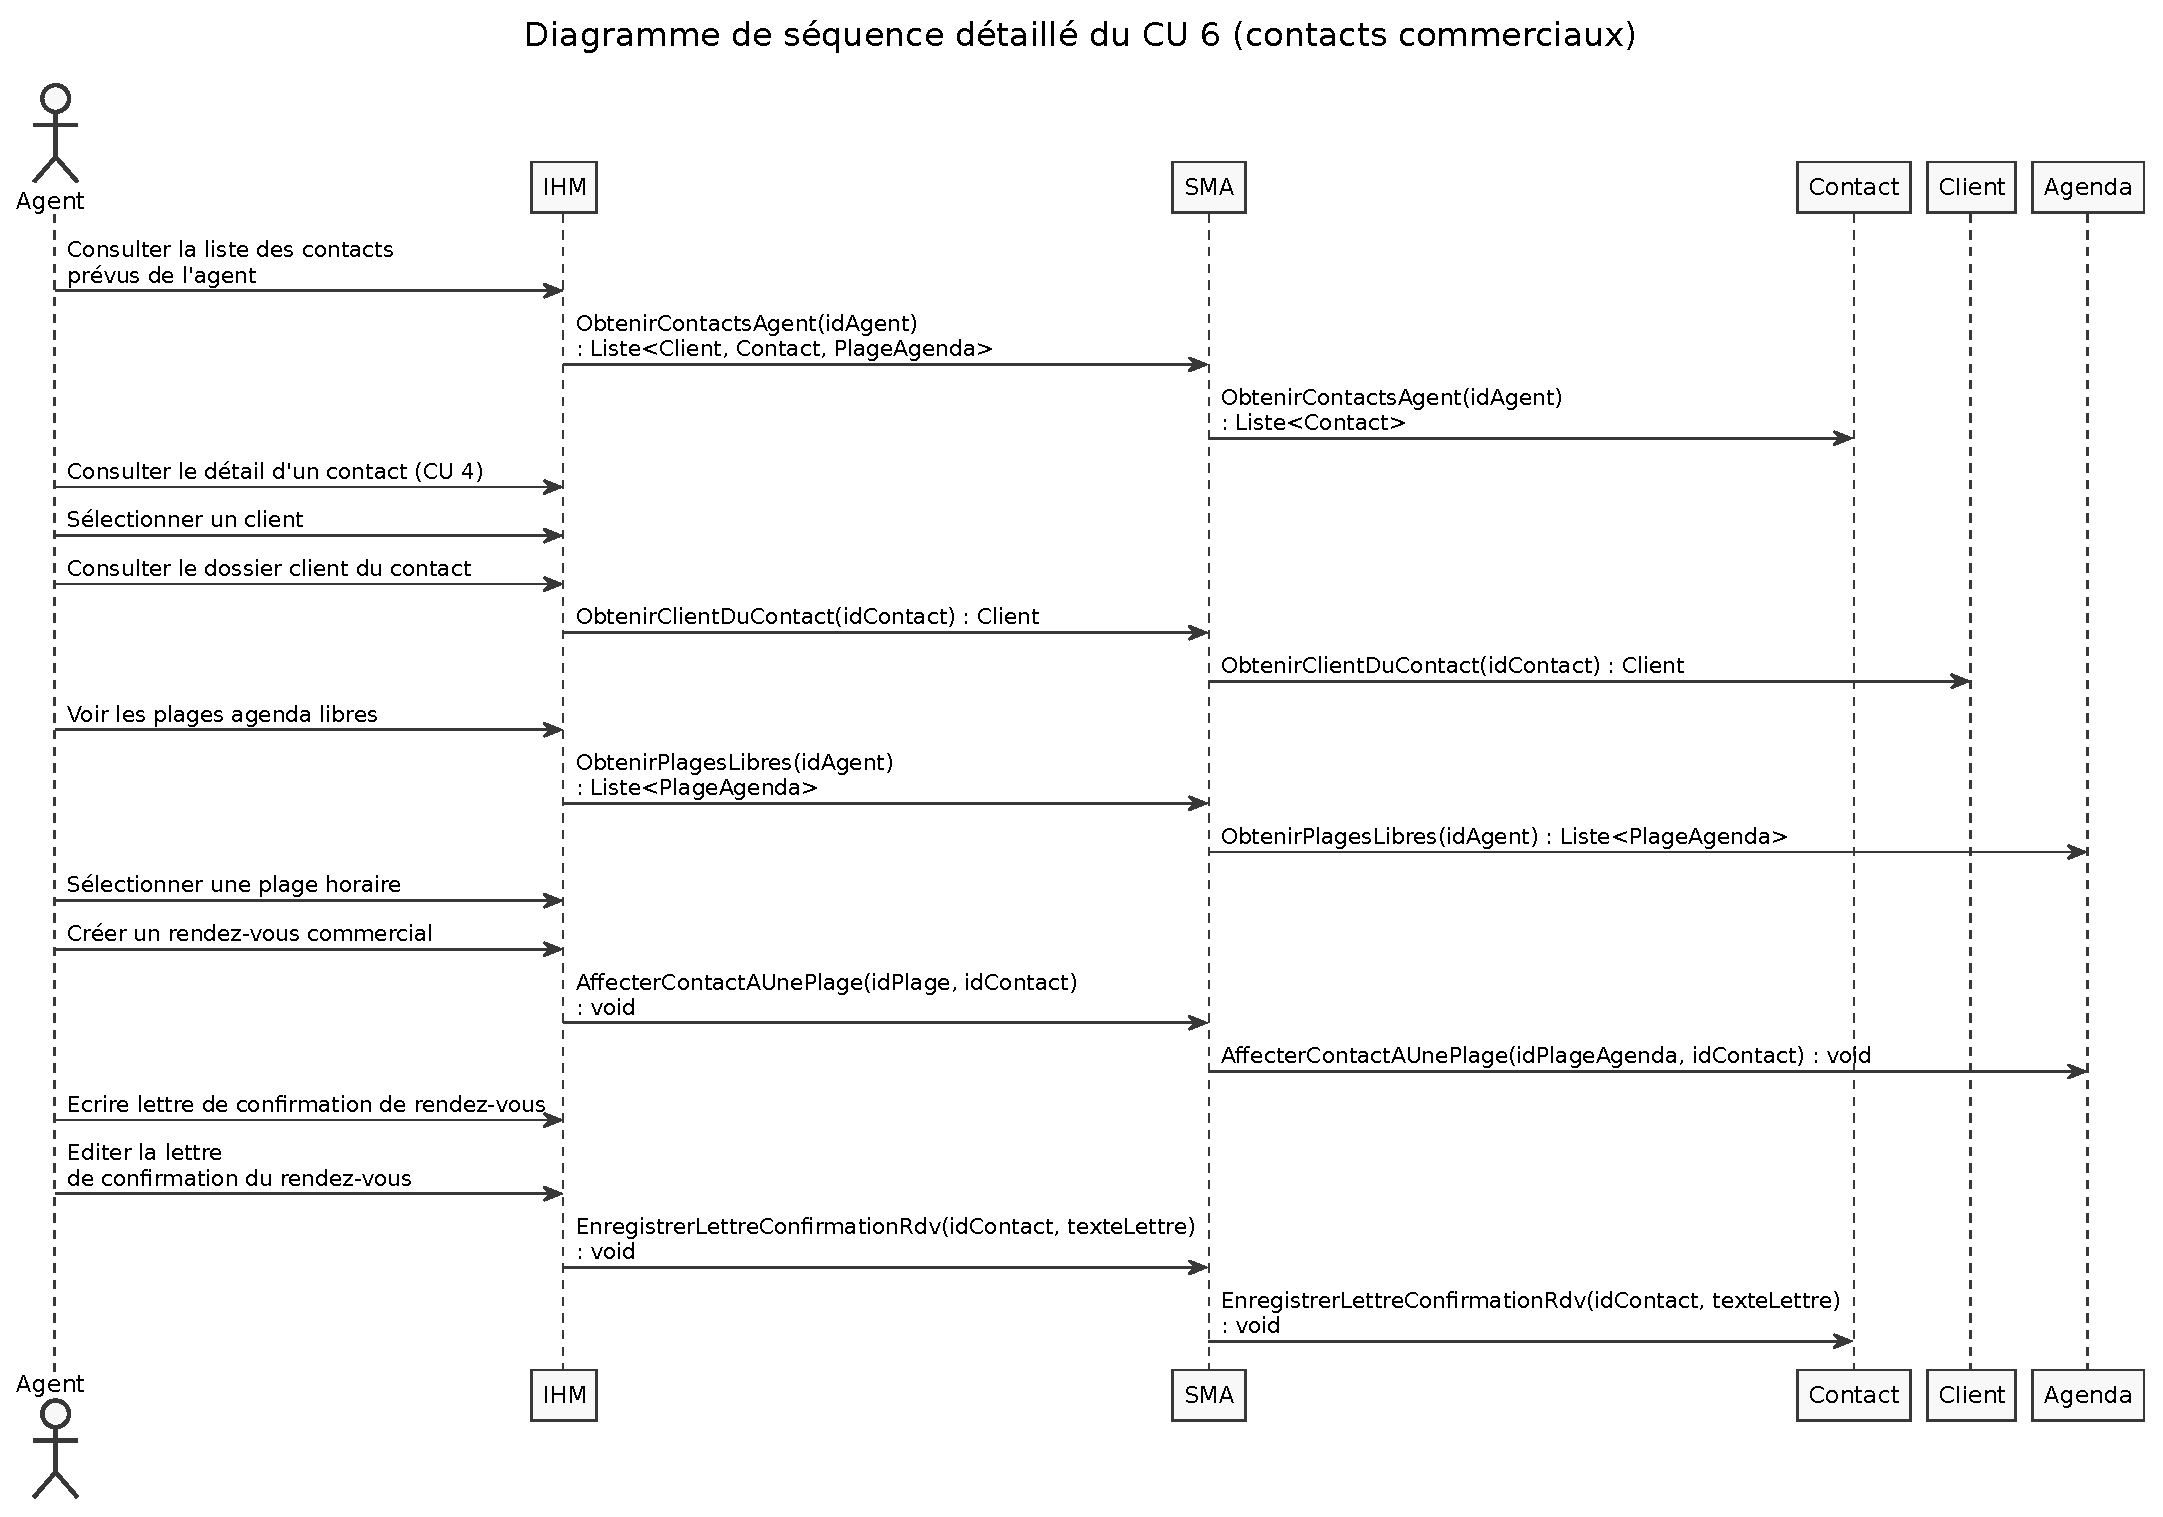
\includegraphics[width=23cm, angle=90]{figures/eps/DSD_CU6_partieAgent.eps}}
\caption{DSD "contacts commerciaux" du CU6}
\end{figure}

\subsubsection{contacts spontanés}
\begin{figure}[H]
\noindent\makebox[\textwidth]{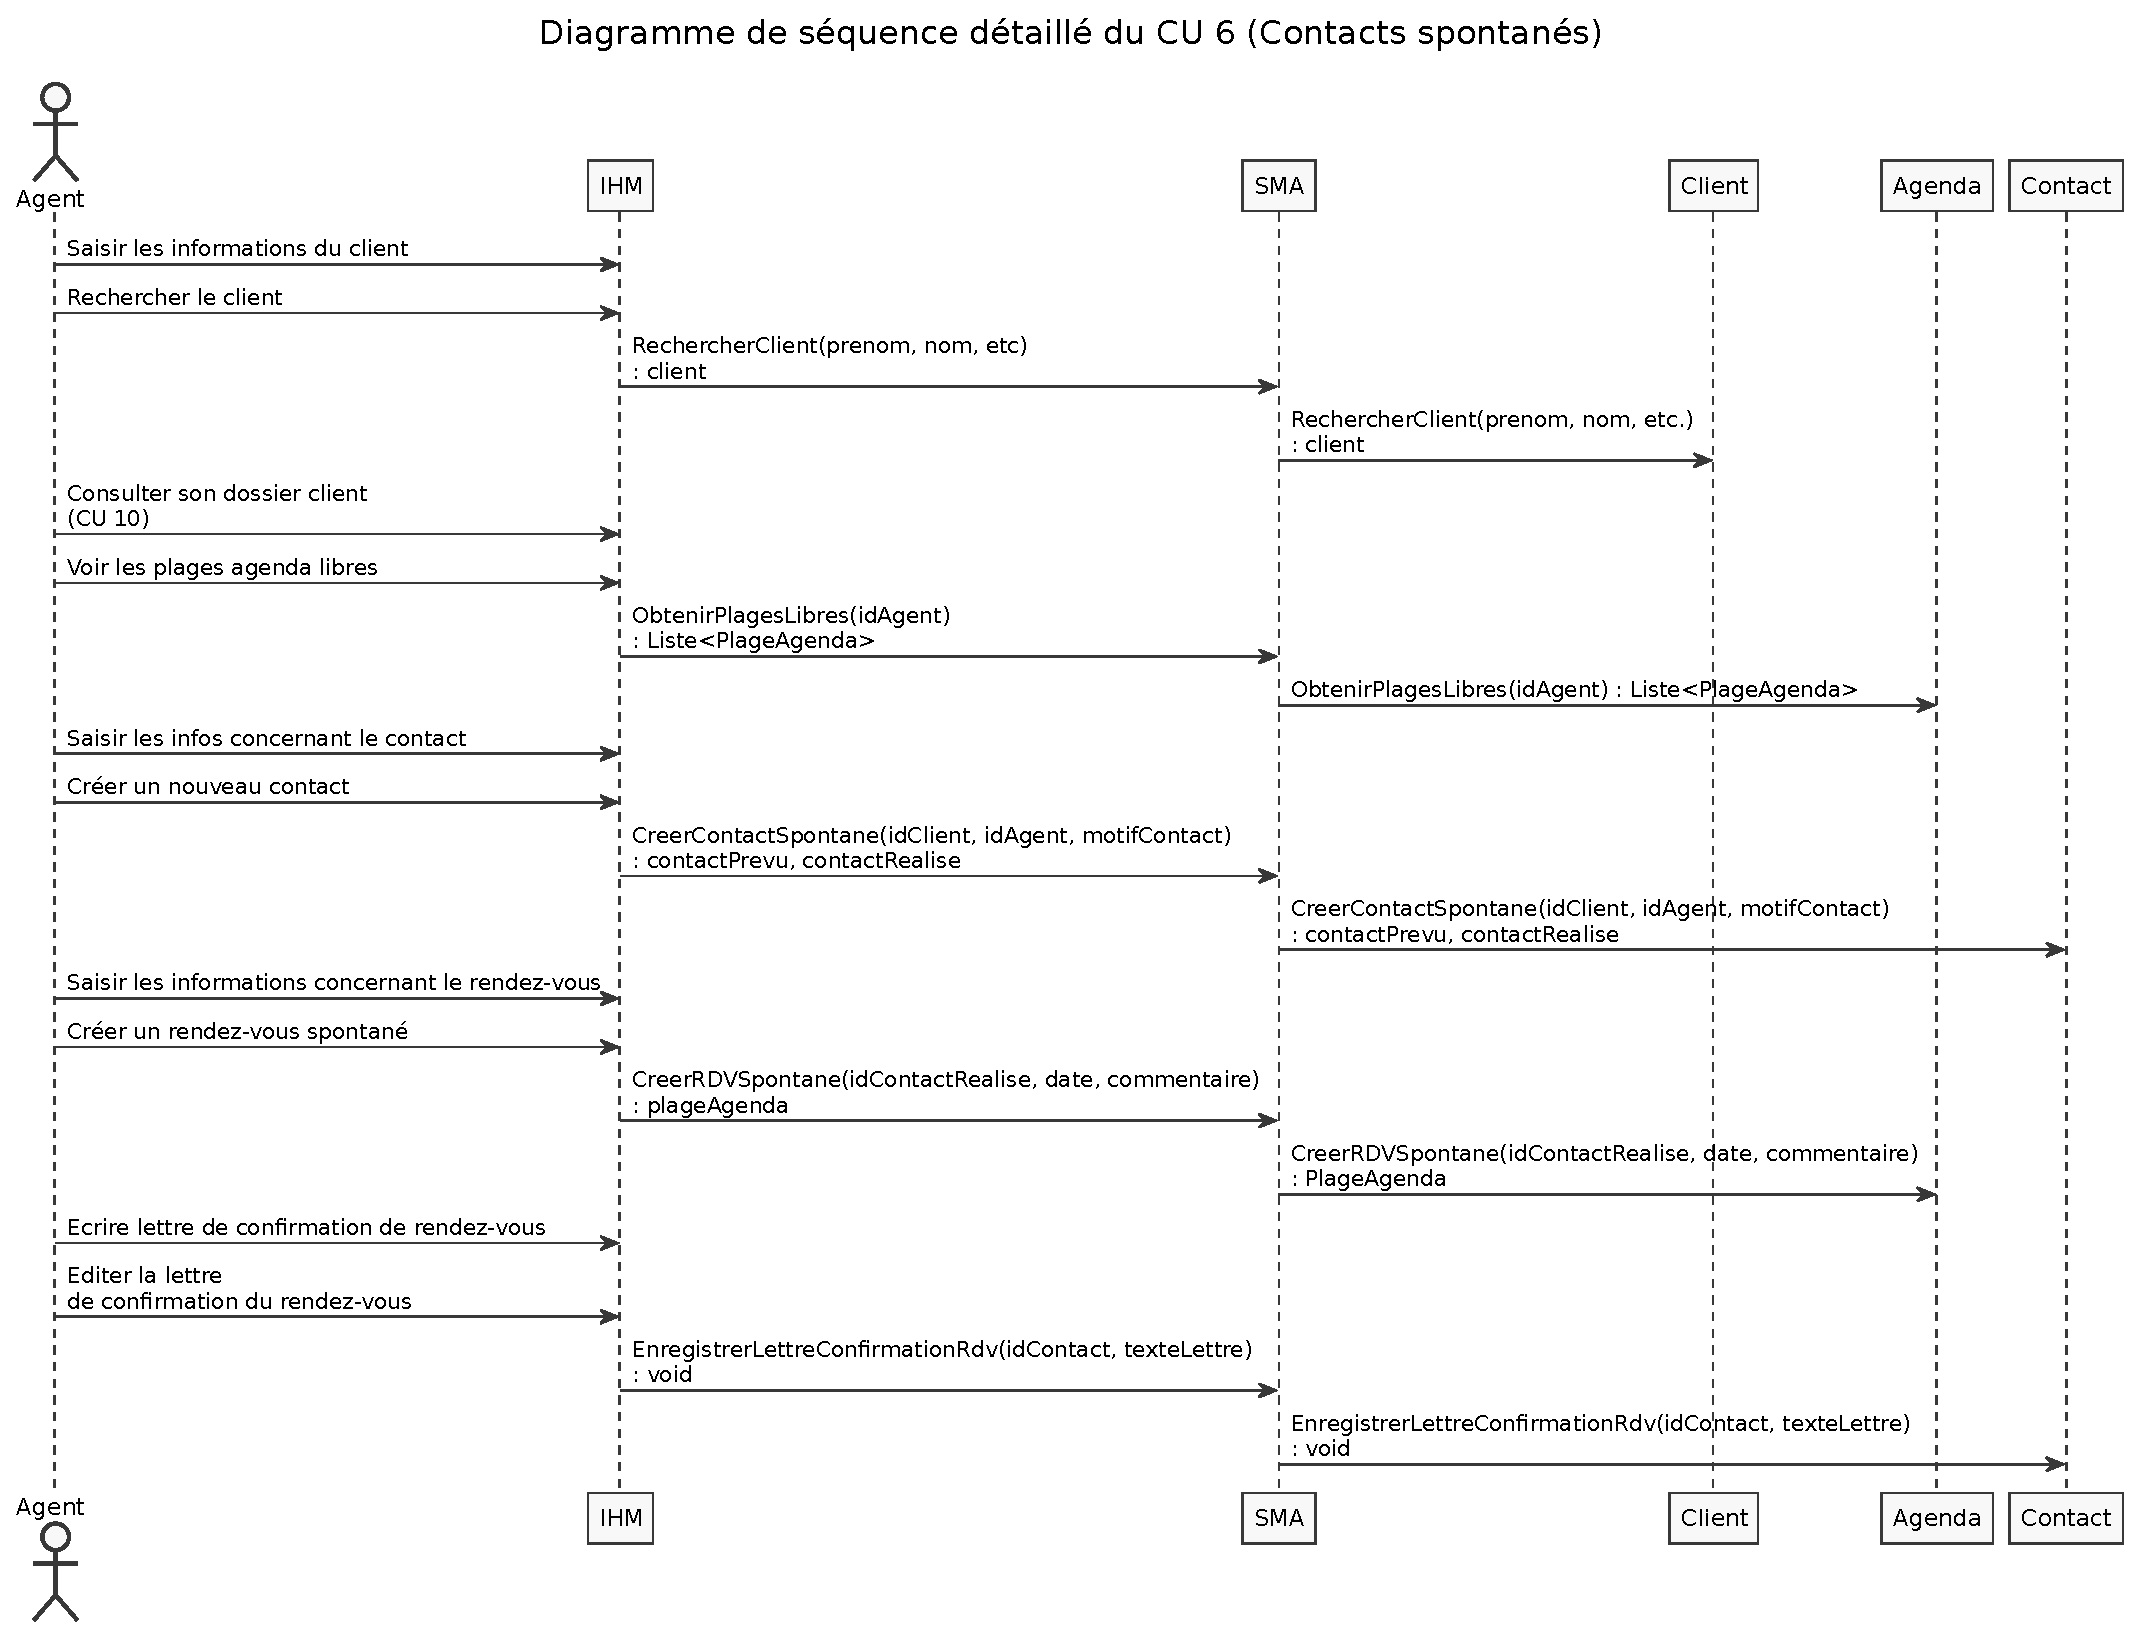
\includegraphics[width=23cm, angle=90]{figures/eps/DSD_CU6_partieClient.eps}}
\caption{DSD "contacts spontanés" du CU6}
\end{figure}


\subsection{CU7 - Consultation des agendas}
\begin{figure}[H]
\noindent\makebox[\textwidth]{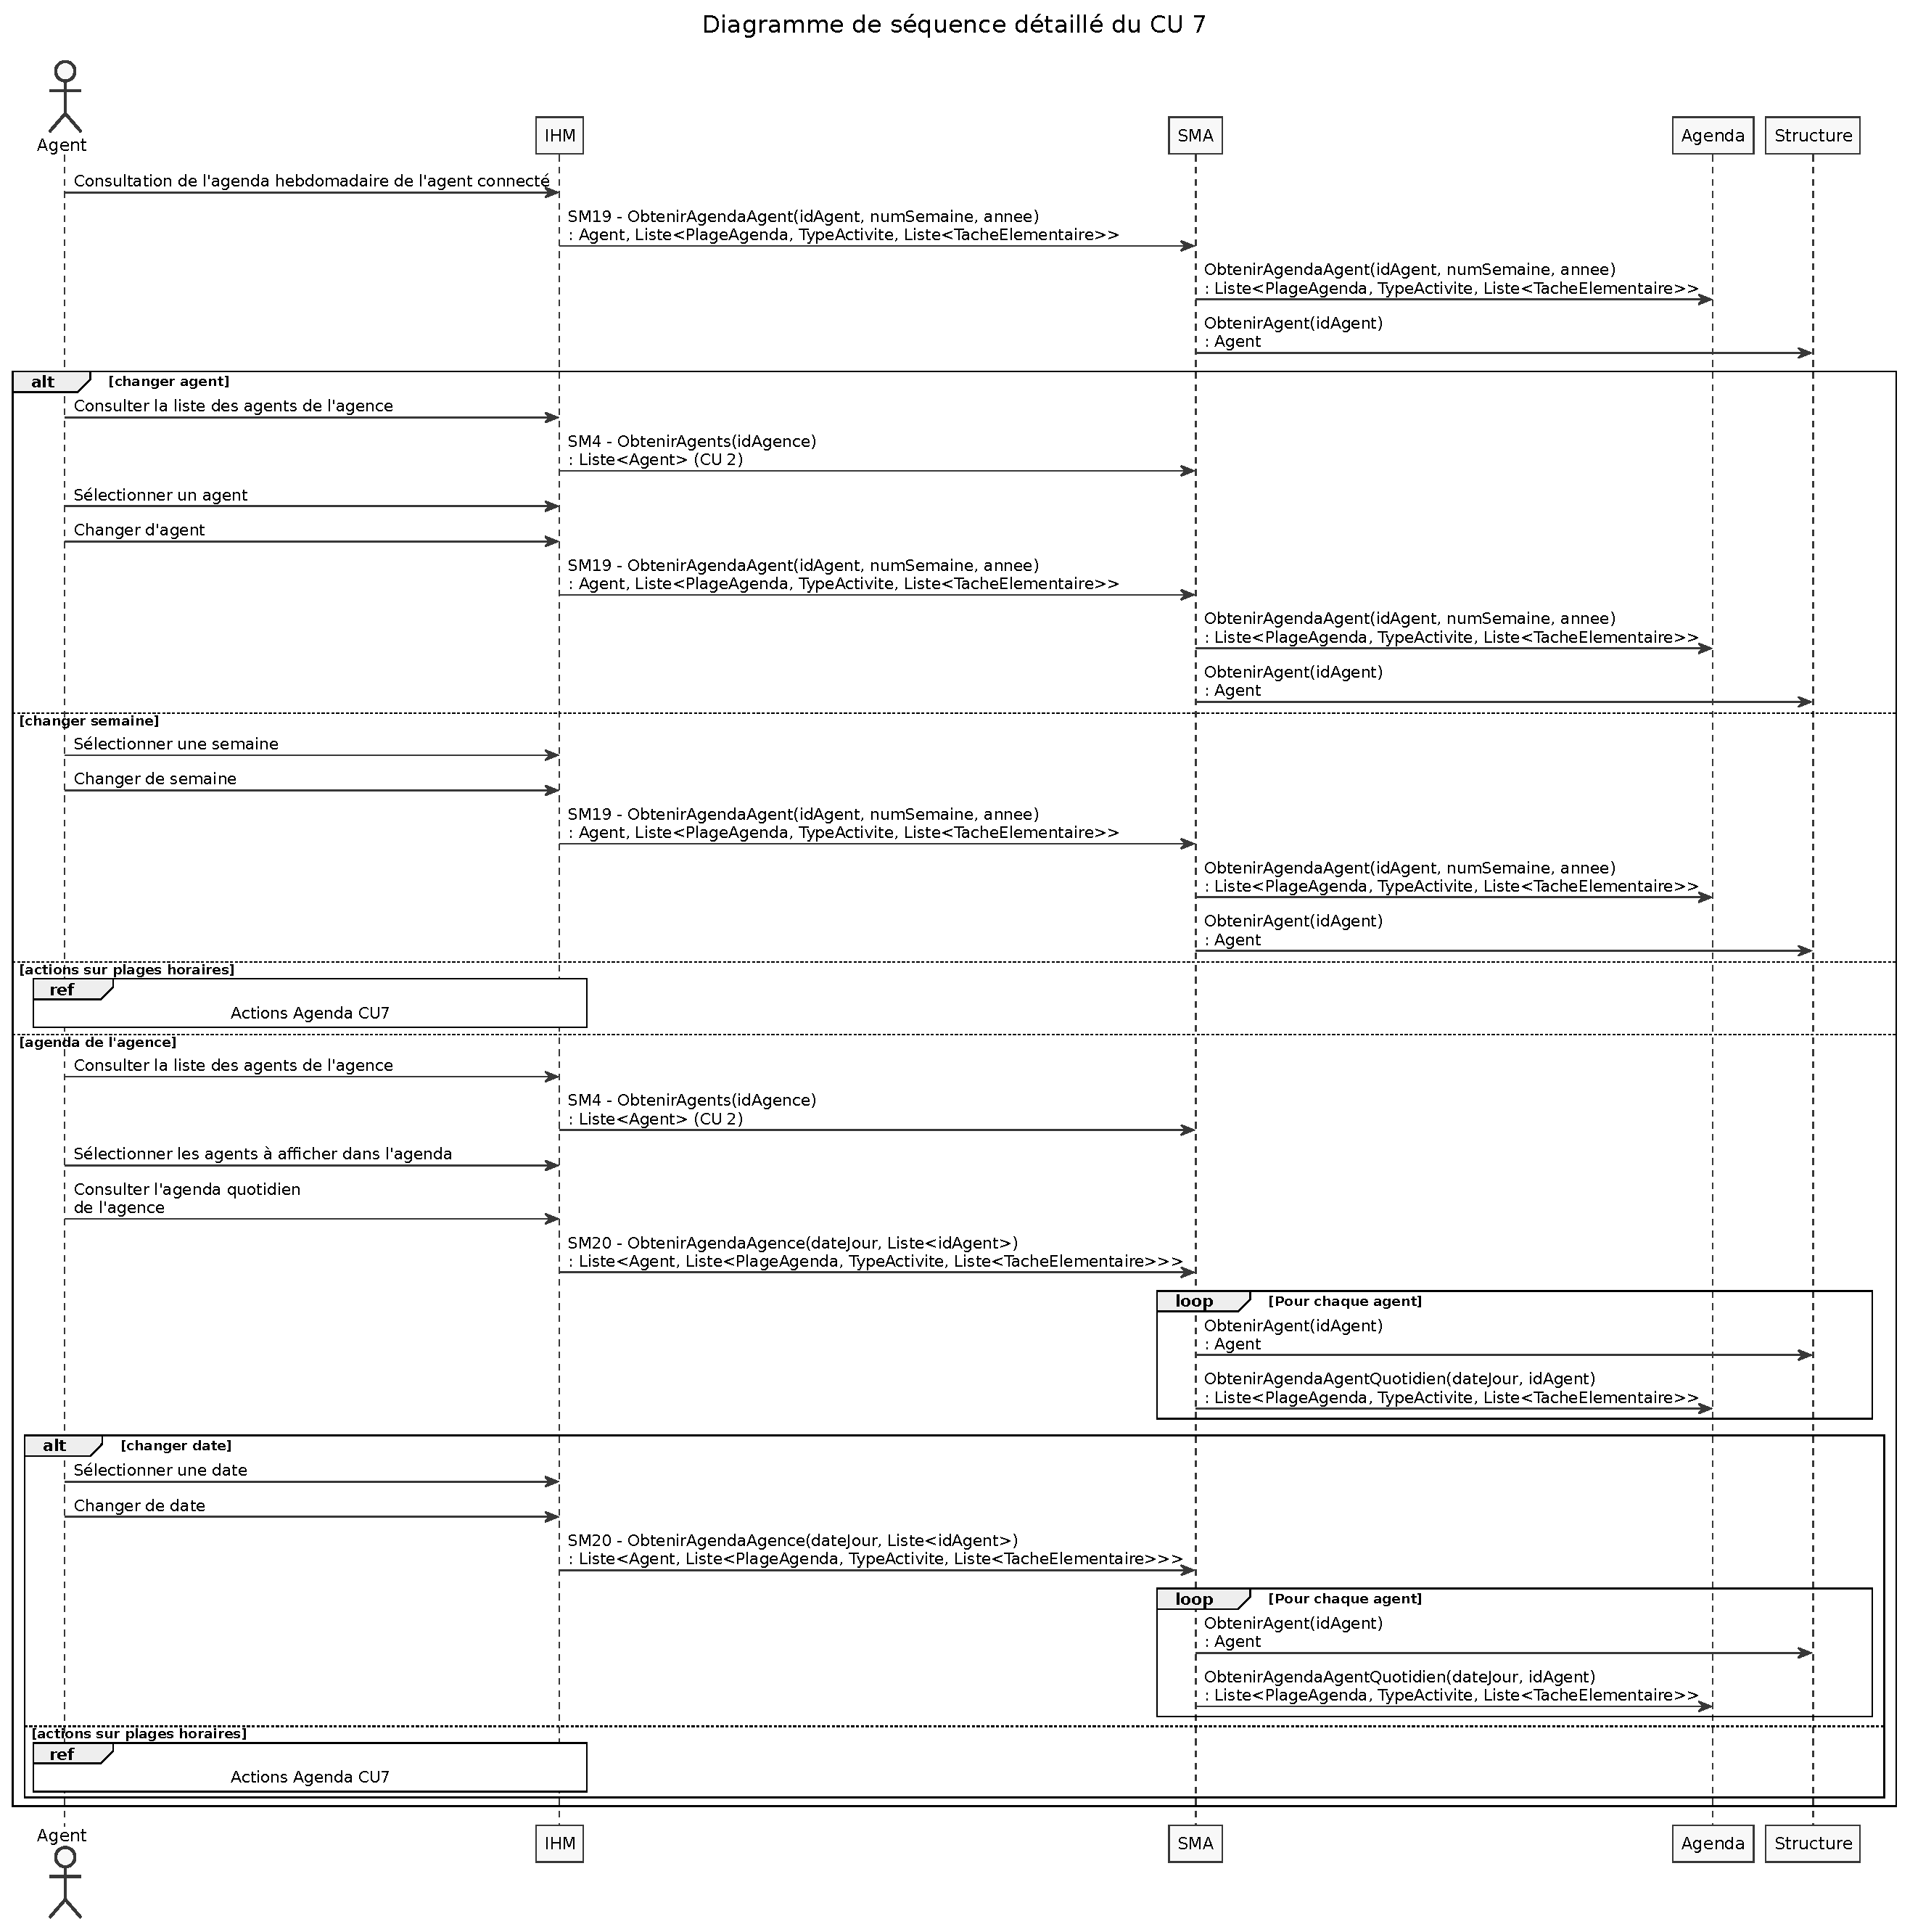
\includegraphics[width=19cm]{figures/eps/DSD_CU7.eps}}
\caption{DSD du CU7}
\end{figure}

\begin{figure}[H]
\noindent\makebox[\textwidth]{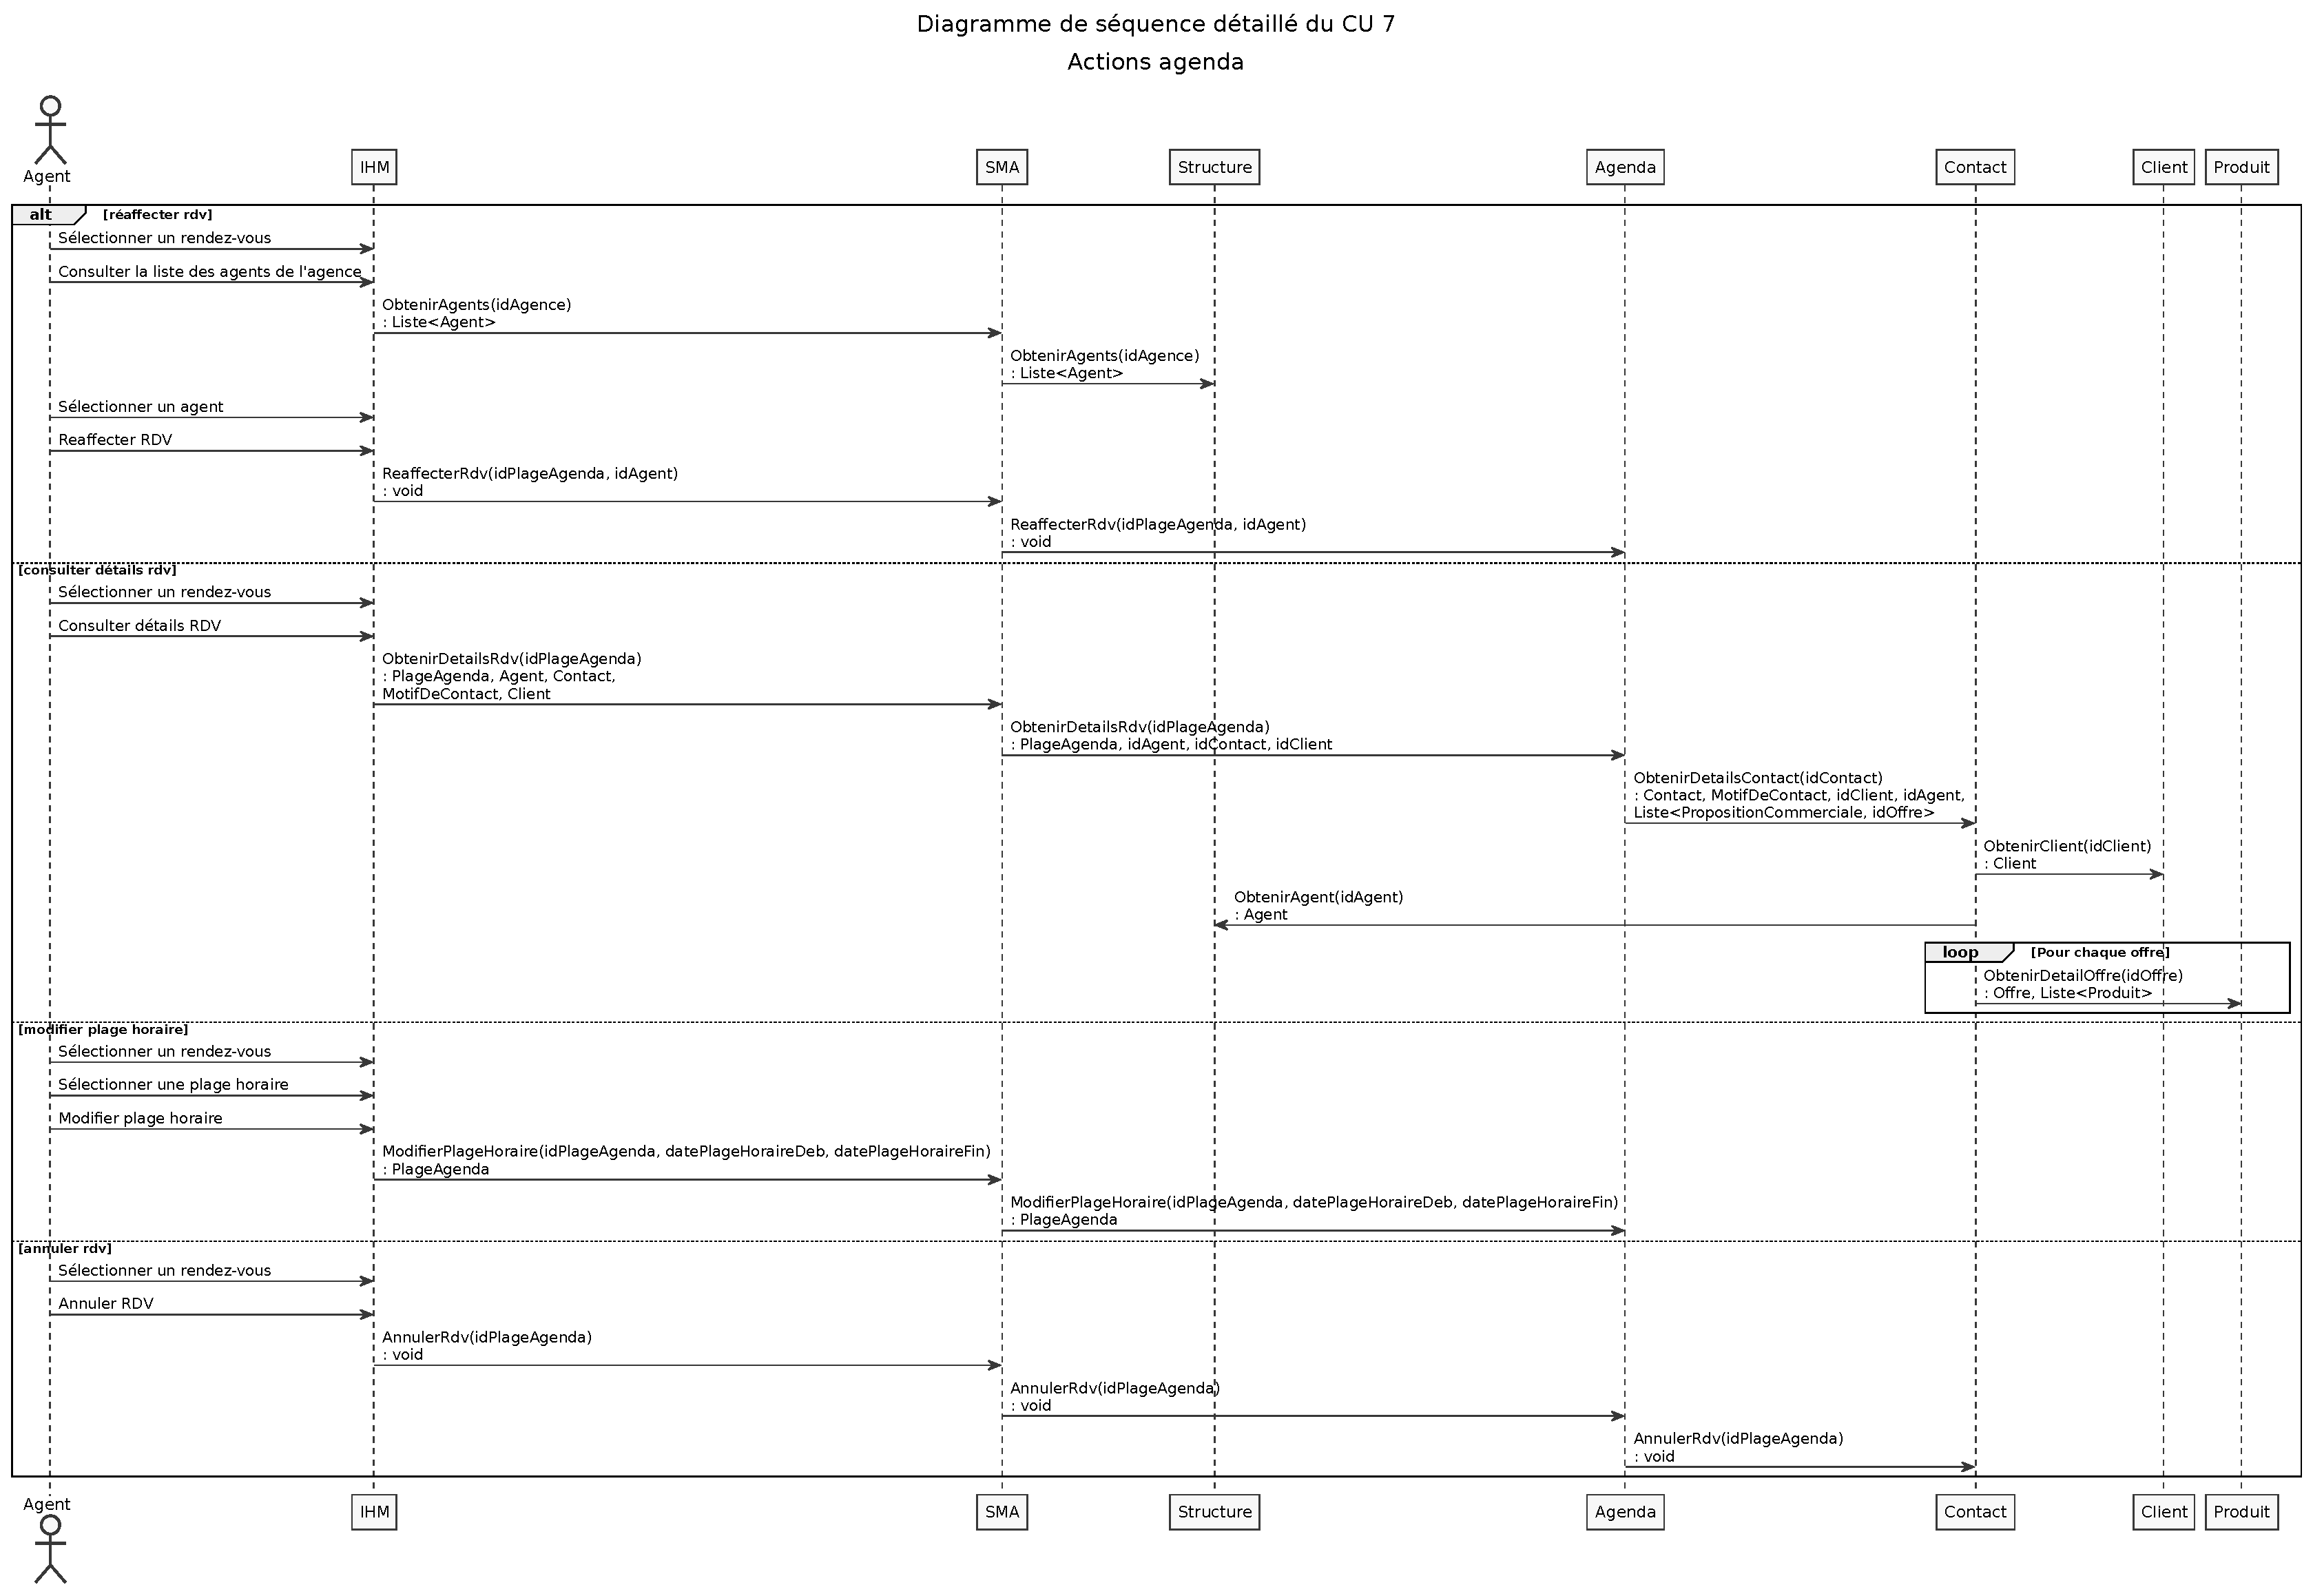
\includegraphics[width=24cm, angle=90]{figures/eps/DSD_CU7_ActionsAgenda}}
\caption{DSD "Actions Agenda" du CU7}
\end{figure}


\subsection{CU8 - Préparation d’entretien par un agent}
\begin{figure}[H]
\noindent\makebox[\textwidth]{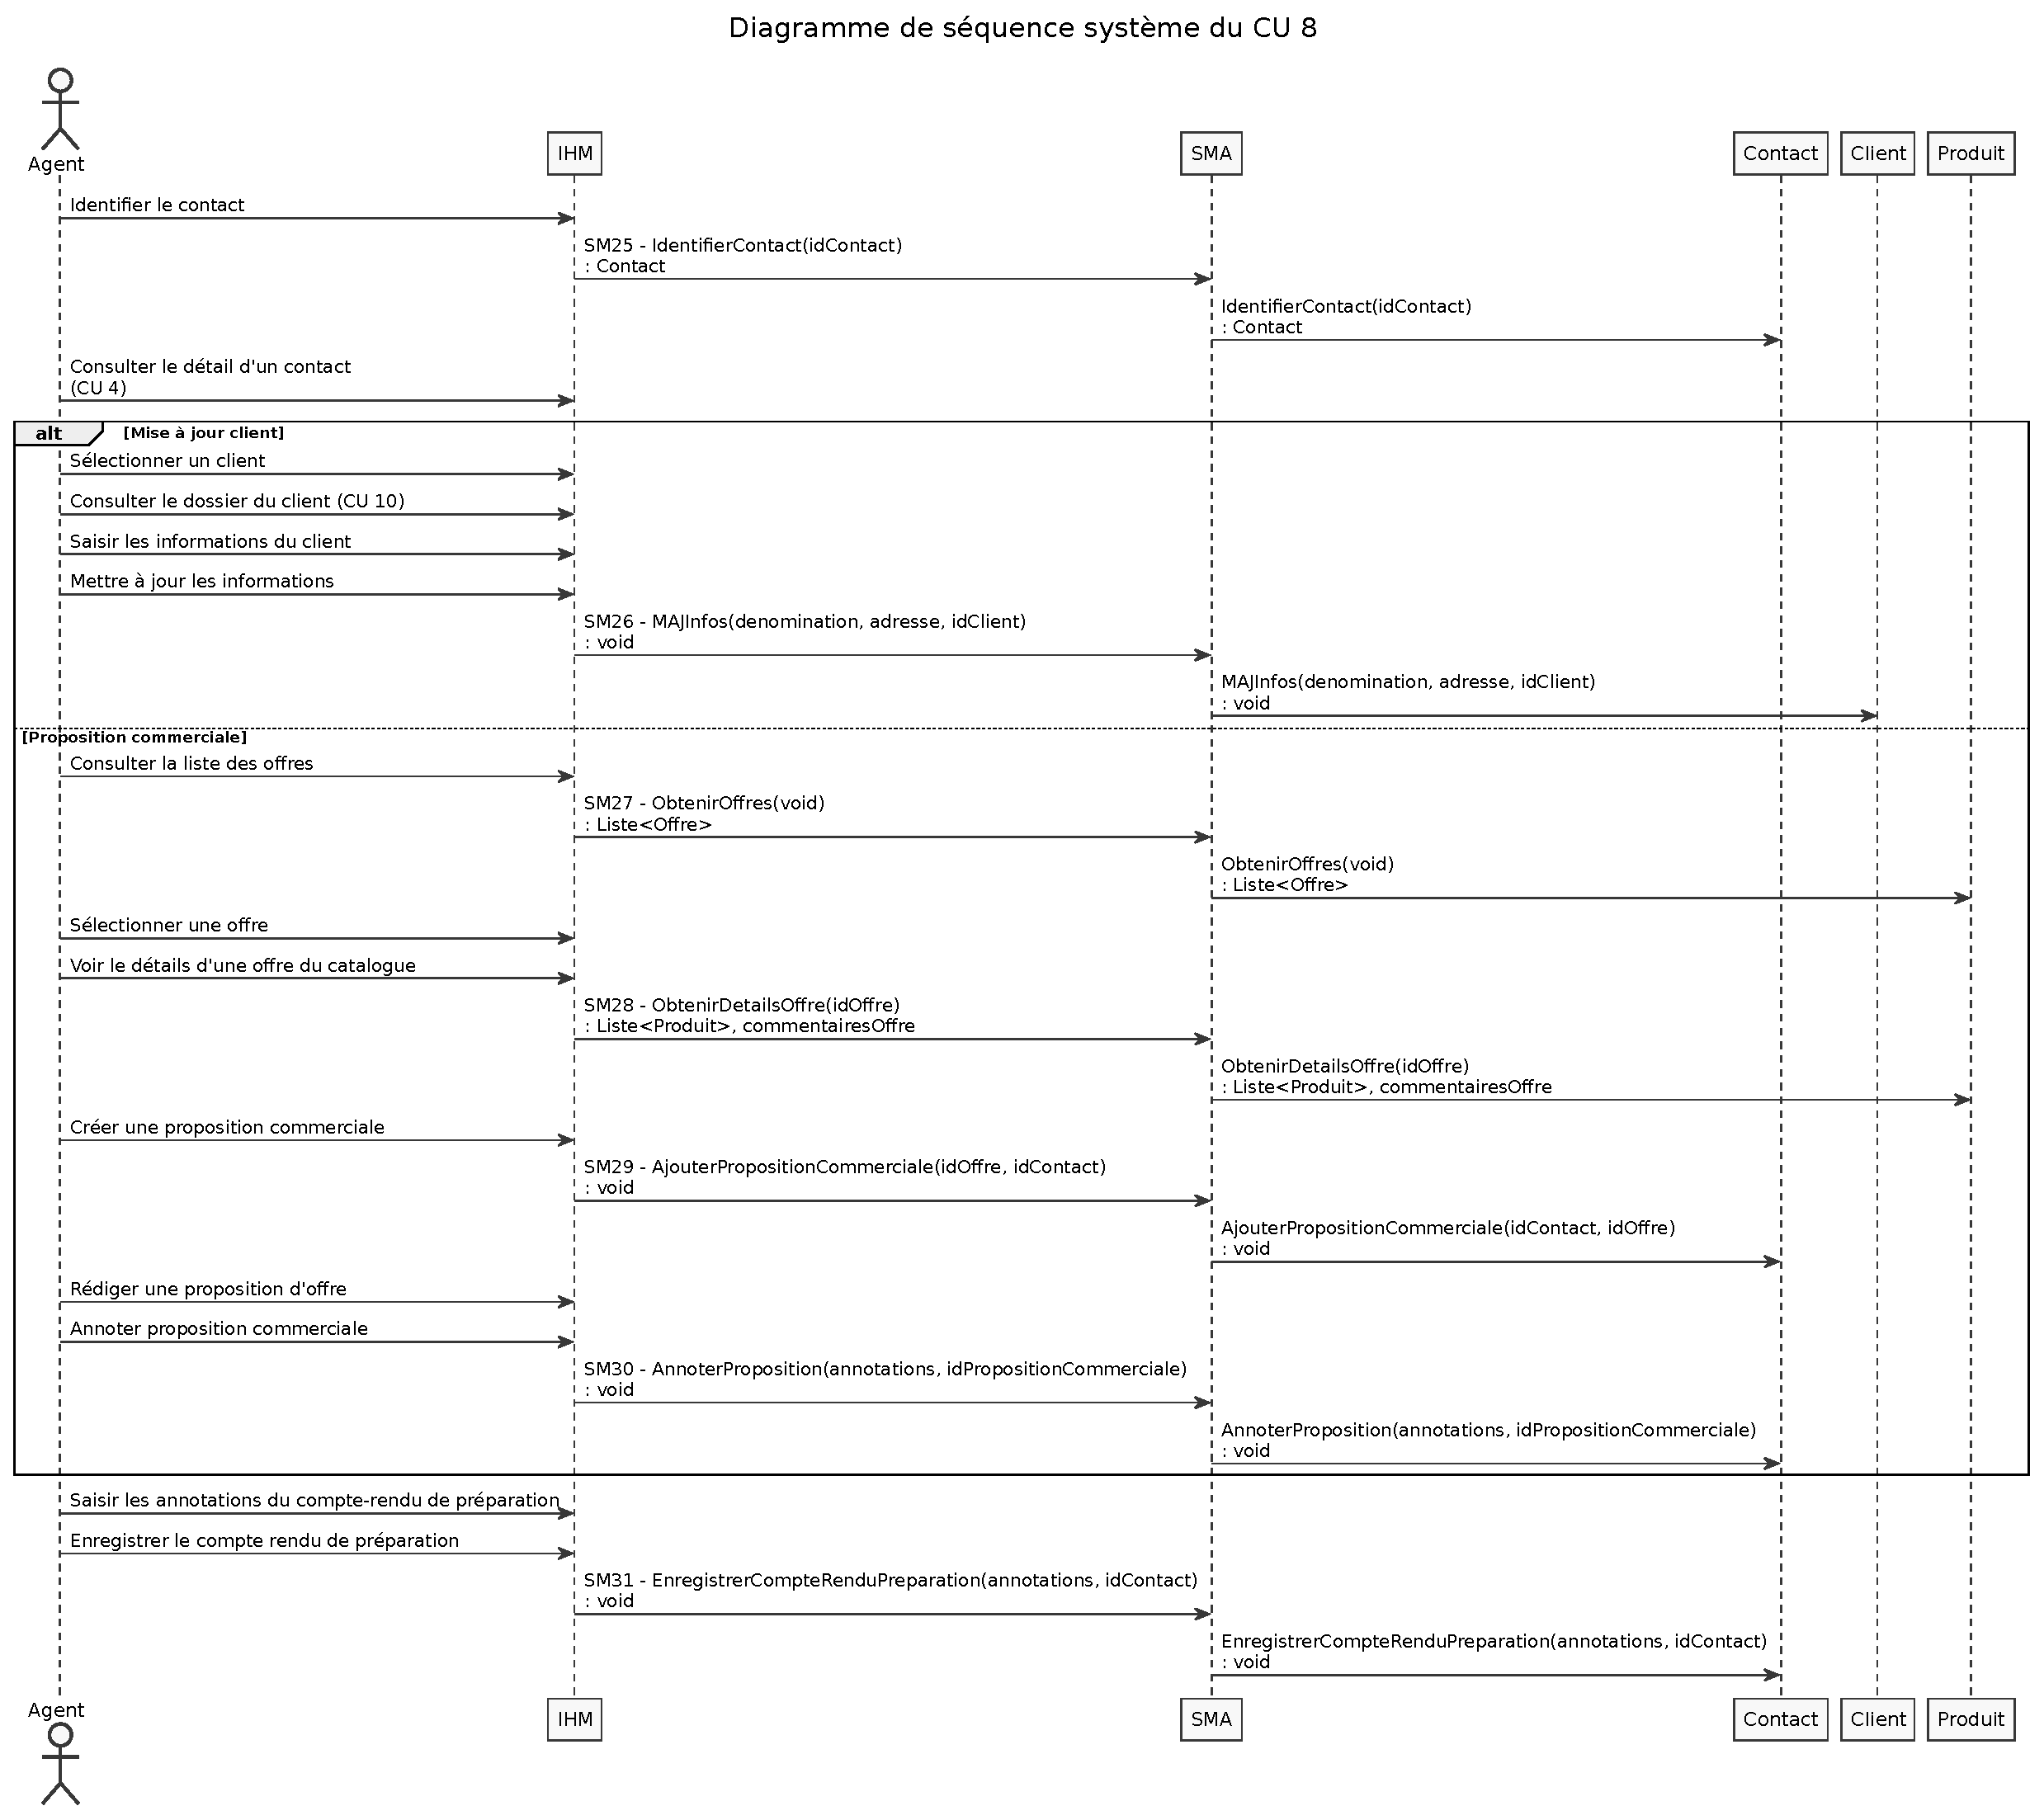
\includegraphics[width=22cm, angle=90]{figures/eps/DSD_CU8.eps}}
\caption{DSD du CU8}
\end{figure}

\subsection{CU9 - Conduite de l’entretien par l’agent}
\begin{figure}[H]
\noindent\makebox[\textwidth]{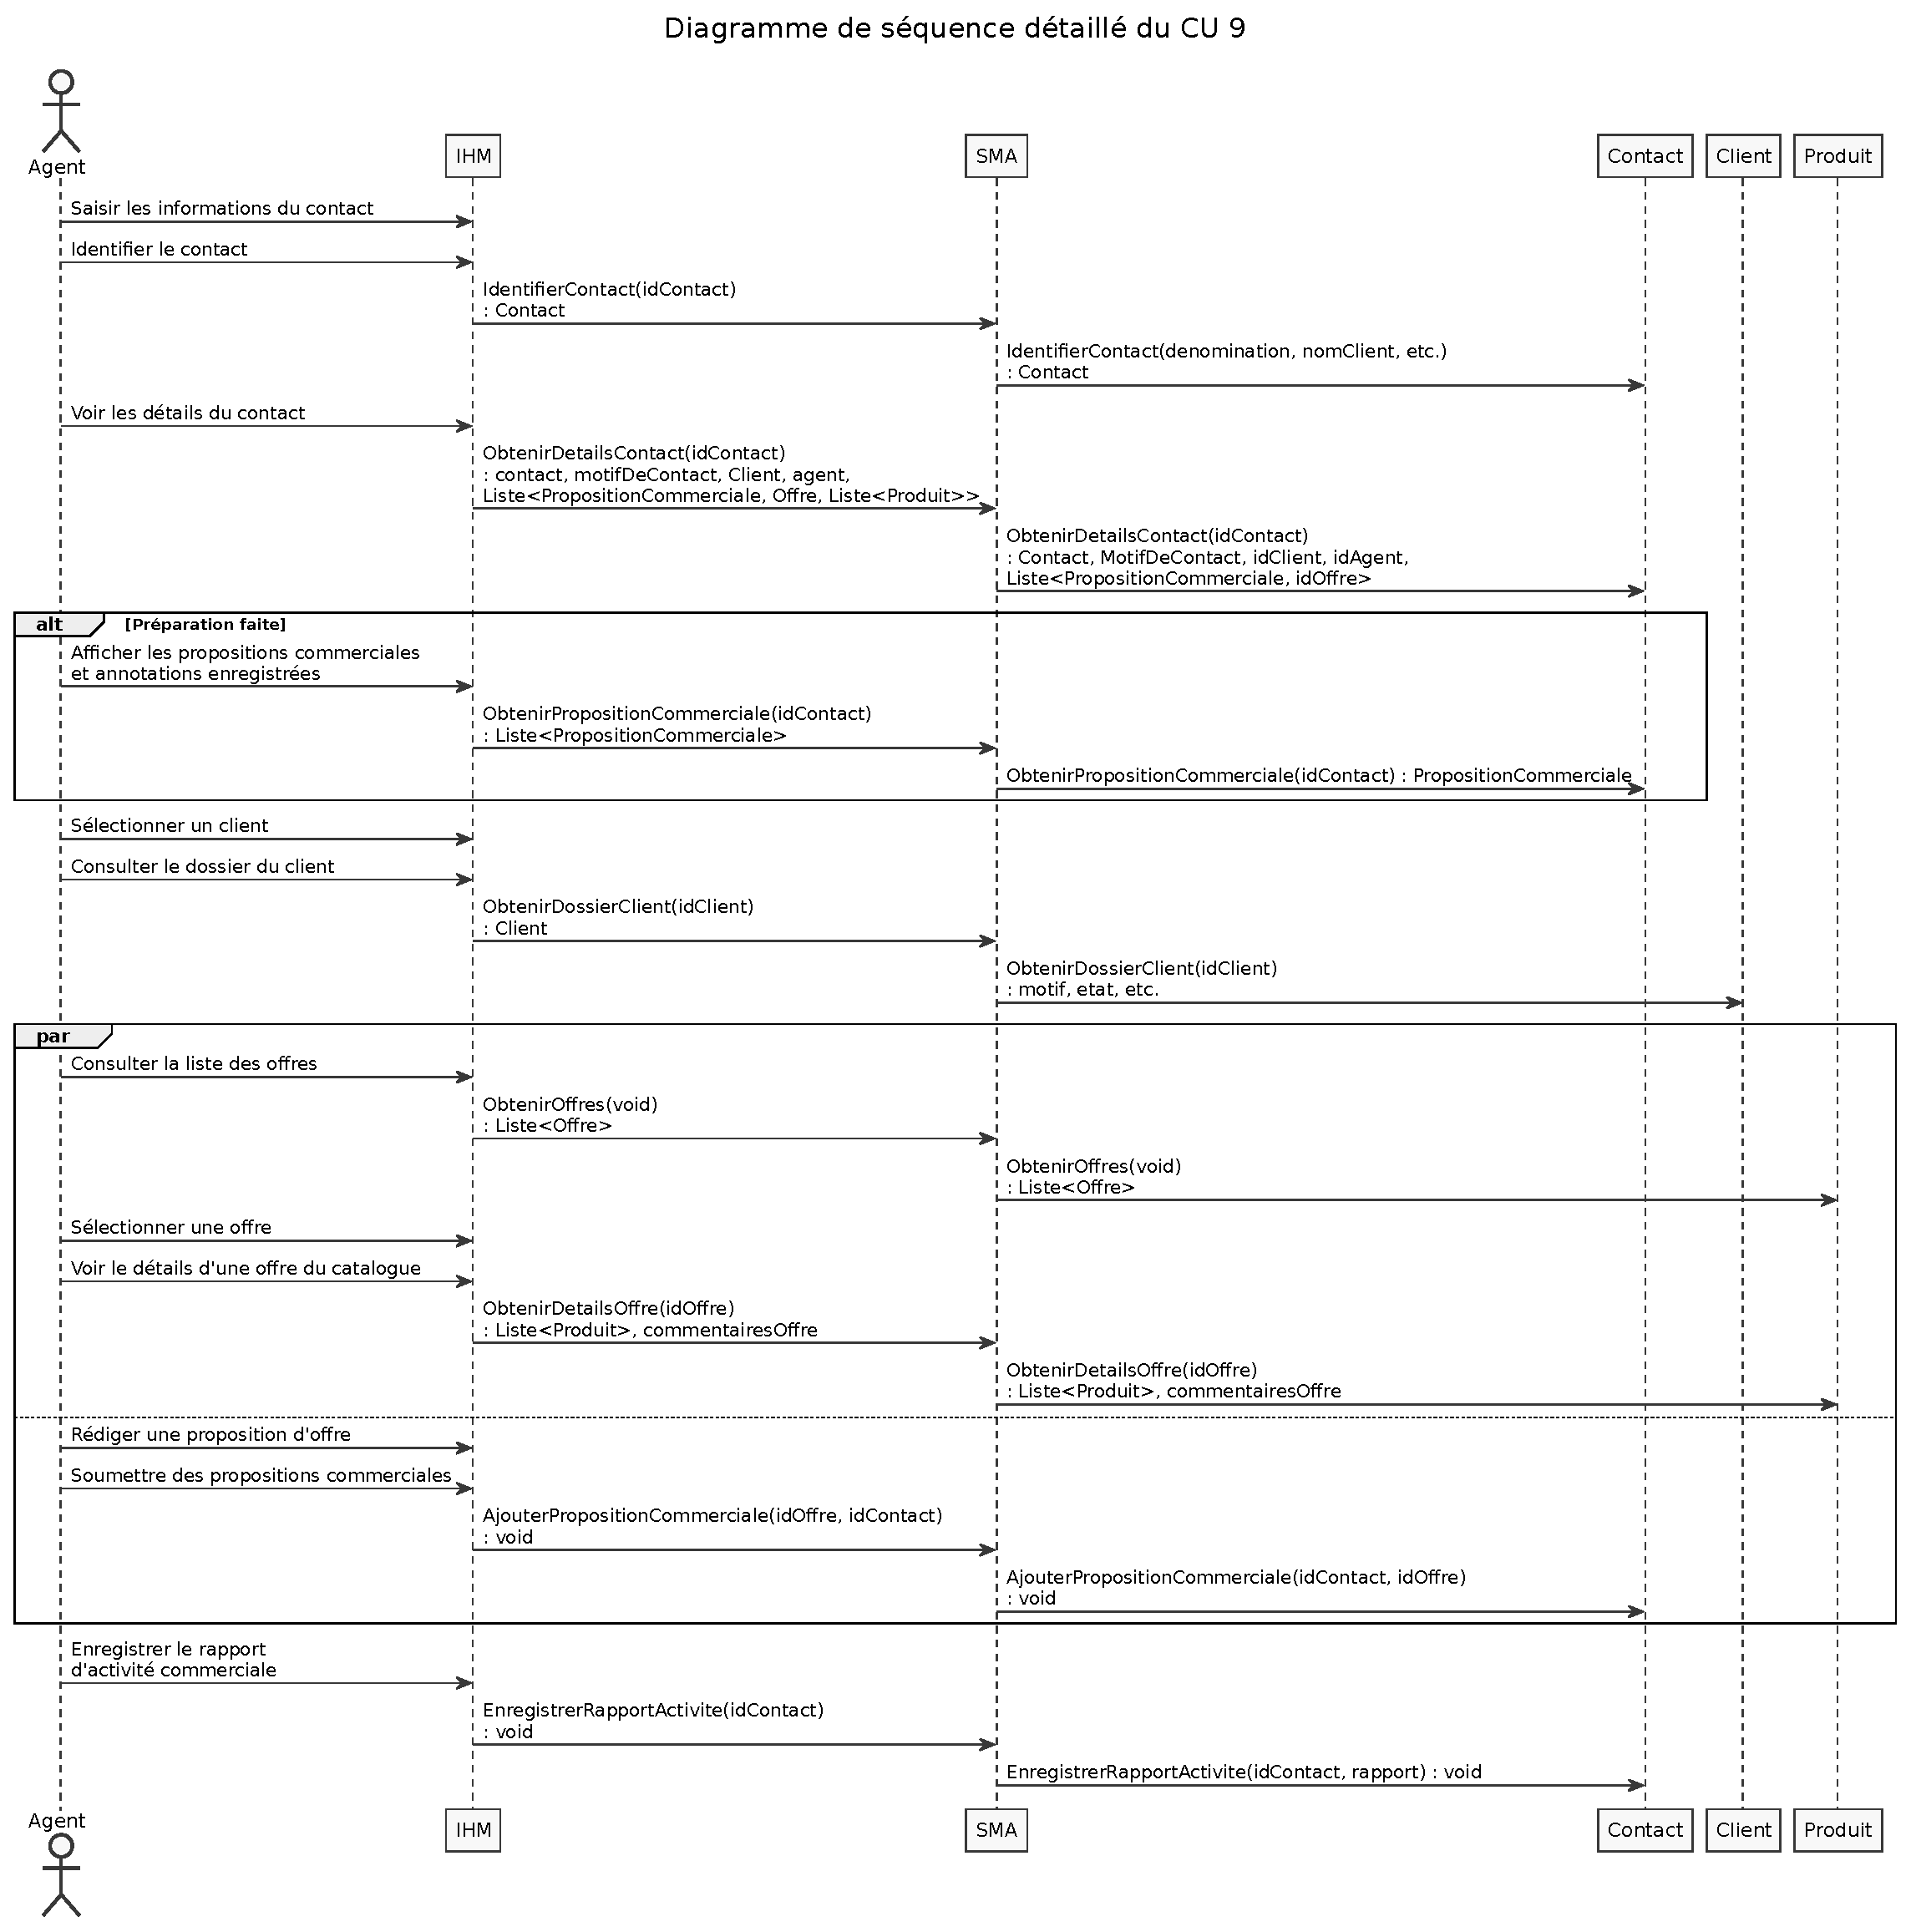
\includegraphics[width=19.5cm, angle=90]{figures/eps/DSD_CU9.eps}}
\caption{DSD du CU9}
\end{figure}

\subsection{CU10 - Consultation du dossier client}
\begin{figure}[H]
\noindent\makebox[\textwidth]{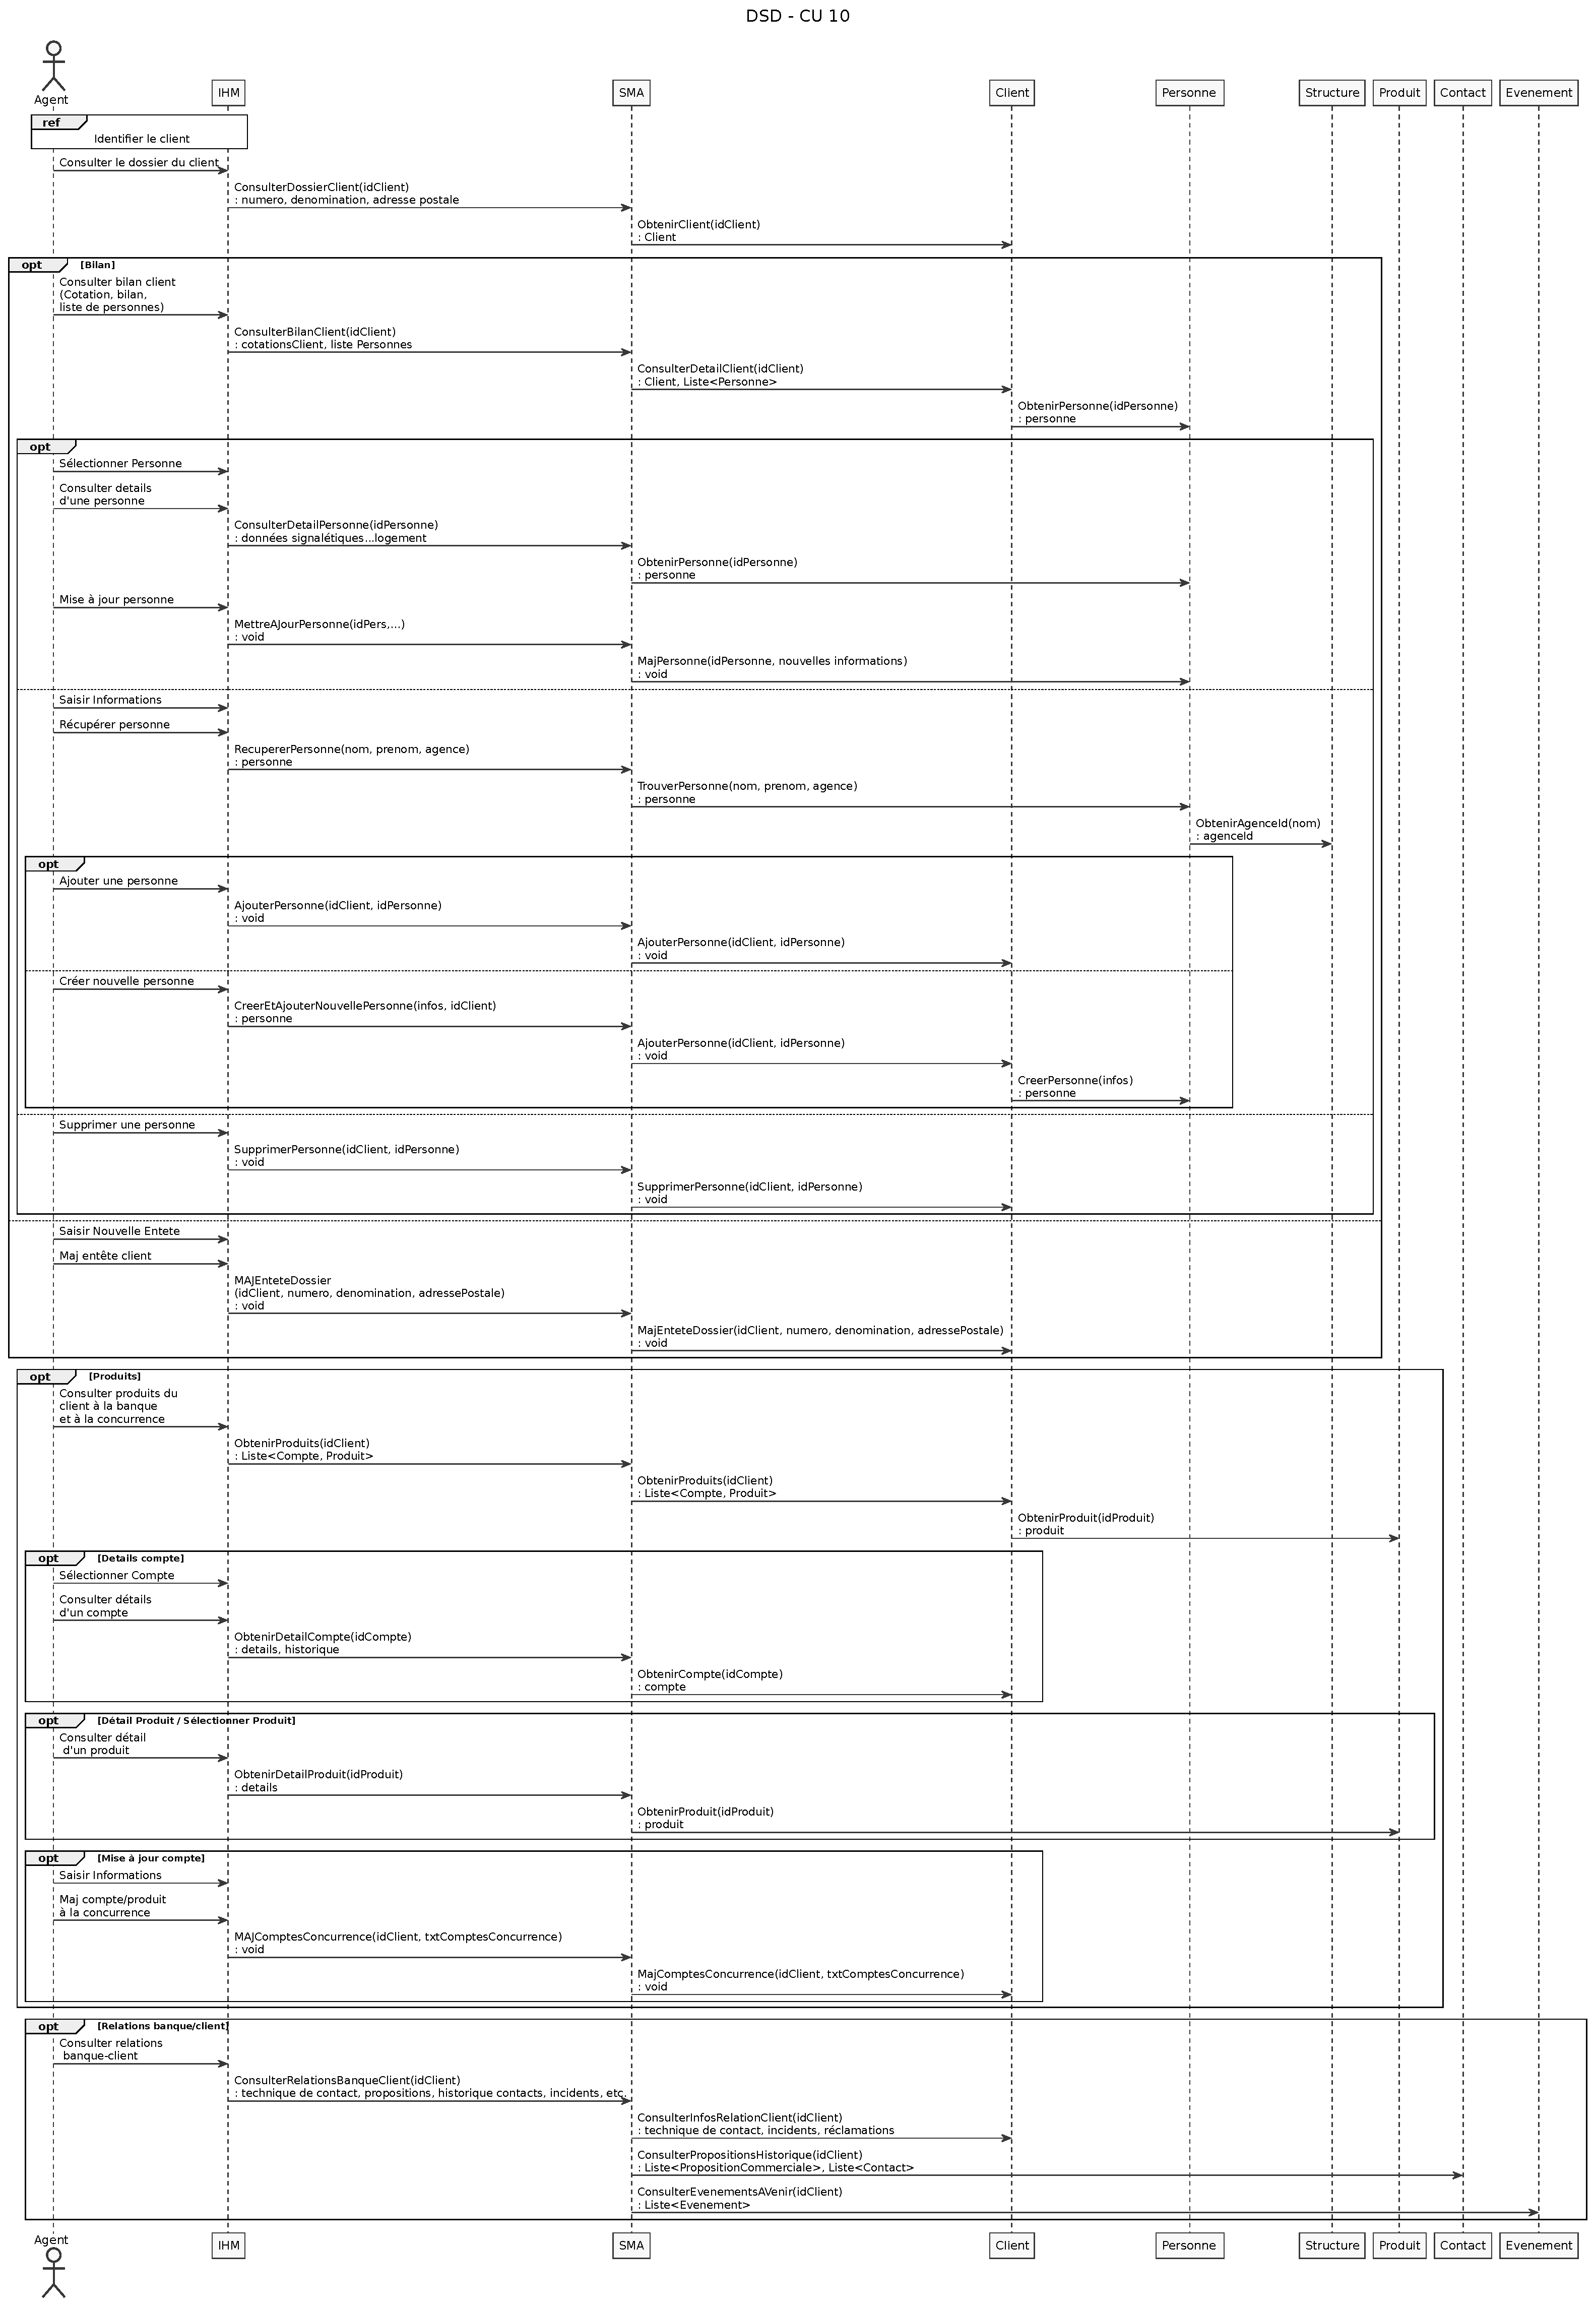
\includegraphics[width=14.2cm]{figures/eps/DSD_CU10.eps}}
\caption{DSD du CU10}
\end{figure}


\newgeometry{height=10in}.
\section{Spécification des services}
\subsection{SMA ObtenirAgendaAgent(idAgent, numSemaine, annee)}
Ce service métier applicatif permet d'obtenir le détail des activités et tâches élémentaires d'un agent pour une semaine en particulier, tout en détaillant les plages horaires associées, permettant ainsi d'obtenir son agenda hebdomadaire. \\

\noindent Arguments en entrée :
\begin{description}
\item[idAgent] l'identifiant numérique de  l'agent pour lequel on souhaite obtenir l'agenda. 
\item[numSemaine] le numéro de la semaine à rechercher, de 1 à 52. 
\item[annee] l'année pour laquelle on souhaite obtenir l'agenda de la semaine mentionnée en second argument, sous format numérique, à quatre chiffres. \\
\end{description}

\noindent Sorties :

\begin{description}
\item[Liste<PlageAgenda>] l'ensemble des plages agenda de l'agent ayant l'identifiant idAgent, pour la semaine numSemaine de l'année annee.
\item[Liste<TacheElementaires>] l'ensemble des tâches élémentaires associées aux plage agenda également retournées. 
\item[Liste<TypeActivite>] l'ensemble des activités de l'agent qui lui sont affectées sur les plage agenda également retournées. \\
\end{description}


\begin{shaded}
SOM associés : Toutes les informations retournées par ce service métier applicatif étant contenues dans le seul bloc Agenda, un seul SOM est nécessaire. De fait, ce dernier dispose de la même signature que le SMA et a pour objectif de récupérer les différentes entités qui correspondent à l'identifiant d'agent spécifié pour la semaine et l'année précisées. 
\end{shaded}

\subsubsection{ObtenirDetailsRdv(idPlageAgenda)} 

Ce service métier applicatif permet de retourner les informations détaillées d'un rendez-vous associé à une plage horaire spécifique.\\

\noindent Arguments en entrée :
\begin{description}
\item[idPlageAgenda] l'identifiant de la plage agenda qui représente le rendez-vous que l'on souhaite détailler. \\
\end{description}

\noindent Sorties : 
\begin{description}
\item[PlageAgenda] : la plage agenda associée à l'identifiant passé en paramètre. 
\item[Agent] l'agent associé à la plage agenda retournée et, de fait, associé au rendez-vous que l'on souhaite détailler. 
\item[Contact] le contact qui est associé à la plage agenda retournée et qui doit être (ou à été) réalisé durant ce créneau horaire.
\item[MotifDeContact] le motif du contact de la plage agenda possédant l'identifiant passé en paramètre. 
\item[Client] le client concerné par le rendez-vous. \\
\end{description}


\begin{shaded}
SOM associés : 
1. Dans un premier temps, le bloc Agenda est interrogé, ce dernier possédant les informations les plus importantes pour ce SMA, ce dernier étant relatif à une plage agenda, qui est une entité de ce bloc. Le service objet métier ci-dessous.
\end{shaded}


\subsubsection{ObtenirDetailsRdv(idPlageAgenda)}

\noindent Arguments en entrée :
\begin{description}
\item[idPlageAgenda] l'identifiant de la plage agenda qui représente de le rendez-vous à détailler. \\
\end{description}

\noindent Sorties : 
\begin{description}
\item[PlageAgenda] la plage agenda présente dans le bloc Agenda, qui correspond à l'identifiant passé en paramètre. 
\item[idAgent] l'identifiant de l'agent associé à la plage agenda, qui sera utilisé pour retrouver l'agent dans le bloc Structure. 
\item[idContact] l'identifiant du contact associé à la page agenda, qui sera utilisé pour retourner le contact et le motif de contact.
\item[idClient] l'identifiant du client relié au contact associé au rendez-vous, qui sera utilisé par le bloc Client à travers le bloc Contact. \\
\end{description}

\begin{shaded}
- 2. Afin d'obtenir les details associés au contact relié à la plage agenda récupérée dans le bloc Agenda,  le bloc Contact est interrogé grâce à l'identifiant contact connu dans le bloc Agenda. Le service objet entier utilisé est le suivant :
\end{shaded}

\subsubsection{ObtenirDetailsContact(idContact)}

\noindent Arguments en entrée :
\begin{description}
\item[idContact] l'identifiant du contact pour lequel on souhaite obtenir les informations détaillées. \\
\end{description}

\noindent Sorties :
\begin{description}
\item[Contact] l'entité contact possédant l'identifiant passé en paramètre. 
\item[MotifDeContact] le motif de contact associé à l'entité contact qui possède l'identifiant passe en paramètre. 
\item[Liste<PropositionCommerciale, idOffre>] l'ensemble des propositions commerciales qui ont été sélectionnées pour le contact également retourné. Si aucune proposition commerciale n'est reliée à ce contact, il s'agit d'une liste vide. Les identifiant des offres associées aux propositions commerciales sont également retournées. 
\item[idClient] l'identifiant du client qui est rattaché à l'entité contact retournée, permettant d'obtenir par la suite plus d'informations sur le client via le bloc Client. \\
\end{description}

\begin{shaded}
- 3. Le bloc Contact ayant permis d'obtenir l'identifiant client associé au contact relié au rendez-vous que l'on souhaite détailler, le bloc Client est ensuite interrogé grâce au service métier suivant :
\end{shaded}

\subsubsection{ObtenirClient(idClient)}

\noindent Arguments en entrée :
\begin{description}
\item[idClient] l'identifiant du client pour lequel on souhaite obtenir plus d'informations. \\
\end{description}


\noindent Sorties :
\begin{description}
\item[Client] l'entité client associée à l'identifiant passée en paramètre et qui correspond au client concerné par le rendez-vous.\\
\end{description}

\begin{shaded}
- 4. Le bloc Contact permettant également d'obtenir l'identifiant de l'agent concerné par le rendez-vous, le service objet métier ci-dessous, du bloc Structure, est ensuite appelé. 
\end{shaded}


\subsubsection{ObtenirAgent(idAgent)}

\noindent Arguments en entrée :
\begin{description}
\item[idAgent] l'identifiant de l'agent qui s'occupe du rendez-vous que l'on souhaite détailler. \\
\end{description}

\noindent Sorties :
\begin{description}
\item[Agent] l'entité agent associé à l'identifiant passé en paramètre et trouvé dans le bloc Structure. \\
\end{description} 

\begin{shaded}
- 5. Enfin, pour chaque offre associée aux propositions commerciales du contact rattaché au rendez-vous, le bloc Produit est interrogé. Cela est dû à l'appel du SOM ObtenirDetailsContact. 
\end{shaded}


\subsubsection{ObtenirDetailOffre(idOffre)}

\noindent Arguments en entrée : 
\begin{description}
\item[idOffre] l'identifiant de l'offre à détailler, qui est associée à une proposition commerciale reliée au contact du rendez-vous. \\
\end{description} 

\noindent Sorties :
\begin{description}
\item[Offre] l'entité offre qui correspond à l'identifiant passé en paramètre, récupéré dans le bloc Produit. 
\item[Liste<Produit>] l'ensemble des produits qui sont reliés à l'offre retournée.
\end{description} 
\restoregeometry


\begin{table}
    \centering
    \scalebox{0.8}{
        \begin{tabular}{p{1cm}|p{5cm}p{6cm}p{6cm}}
            Numéro SM & Nom & Arguments & Valeur de retour \\ \hline
            1  & GenererContacts                    & void                                                          & void \\ \hline
            2  & ObtenirContactsPrevus              & idAgence                                                      & Liste <Contact> \\ \hline
            3  & ObtenirDetailsContact              & idContact                                                     & contact, motifDeContact, client, agentListe<PropositionCommerciale>, Liste<Offre>, Liste<Produit>\\ \hline
            4  & ObtenirDossierClient               & idClient                                                      & Client\\ \hline
            5  & ObtenirAgents                      & idAgence                                                      & Liste<Agent>\\ \hline
            6  & ObtenirDetailsAgent                & idAgent                                                       & agent, Liste<ContactPrevu>\\ \hline
            7  & AffecterContact                    & idContact, idAgent                                            & void\\ \hline
            8  & ObtenirContactsAgent               & idAgent                                                       & Liste<Contact>\\ \hline
            9  & ObtenirContactsATraiter            & idAgent                                                       & Liste<ContactRealise>\\ \hline
            10 & GrouperContacts                    & idContactPrincipal, Liste<idContactPrevus>                    & void\\ \hline
            11 & EnregistrerMotifAnnulation         & idContact, motif                                              & void\\ \hline
            12 & AnnulerContact                     & idContact                                                     & void\\ \hline
            13 & PrendreRdv                         & idContact                                                     & void\\ \hline
            14 & PreparerRdv                        & idContact                                                     & void\\ \hline
            15 & ConduireRdv                        & idContact                                                     & void\\ \hline
            16 & ObtenirAgendaAgent                 & idAgent, numSemaine, annee                                    & Liste<PlageAgenda>, Liste<TacheElementaire>, Liste<TypeActivite> \\ \hline
            17 & ReaffecterRdv                      & idPlageAgenda, idAgent                                        & void\\ \hline
            18 & ObtenirDetailsRdv                  & idPlageAgenda                                                 & plageAgenda, agent, contactRealise,  contactPrevu, motifDeContact, client\\ \hline
            19 & ModifierPlageHoraire               & idPlageAgenda, plageHoraireDeb, plageHoraireFin               & plageAgenda\\ \hline
            20 & ObtenirAgendaAgence                & idAgence, dateJour                                            & Liste<PlageAgenda>, Liste<TacheElementaire>,  Liste<TypeActivite>\\ \hline
            21 & AnnulerRdv                         & idPlageAgenda                                                 & void\\ \hline
            22 & CreerPlageAgenda                   & idAgent, idActivite, datePlageHoraireDeb, datePlageHoraireFin & plageAgenda\\ \hline
            23 & MajNbContactsPotentiels            & idAgent, Liste<idPlageAgenda>                                 & void\\ \hline
            24 & IdentifierContact                  & idContact                                                     & Contact\\ \hline
            25 & MAJInfos                           & saisie, idClient                                              & void\\ \hline
            26 & ObtenirOffres                      & void                                                          & Liste<Offre>\\ \hline
            27 & ObtenirDetailsOffre                & idOffre                                                       & Details\\ \hline
            28 & AjouterPropositionCommerciale      & idOffre, idContact                                            & void\\ \hline
            29 & EnregistrerCompteRenduPreparation  & idContact                                                     & void\\ \hline
            30 & ObtenirPropositionCommerciale      & idContact                                                     & Liste<PropositionCommerciale>\\ \hline
            31 & EnregistrerRapportActivite         & idContact                                                     & void\\ \hline
            32 & ConsulterDossierClient             & idClient                                                      & numero, denomination, adresse postale\\ \hline
            33 & ConsulterBilanClient               & idClient                                                      & cotationsClient, liste Personnes\\ \hline
            34 & ConsulterDetailPersonne            & idPersonne                                                    & données signalétiques...logement\\ \hline
            35 & MettreAJourPersonne                & idPers,...                                                    & void\\ \hline
            36 & RecupererPersonne                  & nom, prenom, agence                                           & personne\\ \hline
            37 & AjouterPersonne                    & idClient, idPersonne                                          & void\\ \hline
            38 & CreerEtAjouterNouvellePersonne     & infos, idClient                                               & personne\\ \hline
            39 & SupprimerPersonne                  & idClient, idPersonne                                          & void\\ \hline
            40 & MAJEnteteDossier                   & idClient, numero, denomination, adressePostale                & void\\ \hline
            41 & ObtenirDetailCompte                & idCompte                                                      & details, historique\\ \hline
            42 & ObtenirDetailProduit               & idProduit                                                     & details\\ \hline
            43 & ObtenirProduits                    & idClient                                                      & Liste<Compte, Produit>\\ \hline
            44 & MAJComptesConcurrence              & idClient, txtComptesConcurrence                               & void \\ \hline
            45 & ObtenirPlagesLibres                & idAgent                                                       & Liste<PlageAgenda>\\ \hline
            46 & AssocierPlageEtContact             & idPlage, idContact                                            & void\\ \hline
            47 & EnregistrerLettreConfirmationRdv   & idContactRealise, lettre                                      & void\\ \hline
            48 & RechercherClient                   & prenom, nom, etc                                              & client\\ \hline
            49 & CreerContactSpontane               & idClient, idAgent, motifContact                               & contactPrevu, contactRealise\\ \hline
            50 & CreerRDVSpontane                   & idContactRealise, date, commentaire                           & plageAgenda \\ \hline 
            51 & ConsulterRelationsBanqueClient & idClient & technique de contact, propositions, historique contacts, incidents, etc. \\ \hline
            52 & ObtenirListeAgence & void & Liste<Agence> \\
        \end{tabular}
        }
        \caption{Tableau de synthèse des SMA}
\end{table}


\begin{table}
    \centering
    \begin{tabular}{l|l}
    Nom de la vue   & Numéros des SMA appelés   \\ \hline
    Page d'authentification & -- \\
    Onglet Client & 52, RechercherClient (?)\\
    Resultat recherche client & 52, RechercherClient (?), 32\\
    Onglet Bilan dossier client & 33\\
    Onglet Produit & \\
    Onglet Relations & \\
    Onglet Agenda & \\
    Mode Agence & \\
    Mode Agent & \\
    Popup d'ajout d'activite & \\
    Popup d'ajout d'un contact commercial & \\
    Popup d'ajout d'un contact spontane & \\
    Popup de selection d'un contact & \\
    Popup de selection d'un client & \\
    Popup d'ajout d'une tâche & \\
    Popup de consultation d'une tache & \\
    Onglet Personnes & \\
    Onglet Contacts & \\
    Dossier Editable & \\ 
    Dossier Non Editable & \\
    Mode Consultation & \\
    Mode Planification & \\
    Liste des contacts & \\
    Vue Contact & \\
    Onglet preparation  & \\
    Onglet compte-rendu & \\
    Popup d'affectation d'un agent au contact & \\
    Popup d'ajout d'une offre & \\
    Liste des personnes & \\
    Vue donnant les détails d'une personne  & \\
    \end{tabular}
    \caption{Tableau de synthèse des SMA par fenêtre}
\end{table}




